\chapter{Marco teórico}
\label{ch:marco}

%%%%%%%%%%%%%%%%%%%%%%%%%%%%%%%%%%%%%%%%%%%%%%%%%%%%%%%%%%%%%%%%%%%%%%%%%%%%%%%%%%%%%%%%%%%%%
 
\section{Lógica reconfigurable y FPGAs}
\subsection{Concepto de lógica reconfigurable}
El hardware reconfigurable es una herramienta en ocasiones subestimada debido a su simplicidad de uso, sin embargo, la complejidad detrás de la lógica reconfigurable, las interconexiones de los módulos que la implementan no son rudimentarias. No funciona mediante instrucciones previamente cargadas, su funcionamiento es estructural, el comportamiento deseado se describe, esa descripción luego es traducida a una cadena de valores lógicos altos y bajos que se almacena secuencialmente en una memoria. Se cuenta con una memoria la cual almacena valores que se pueden interpretar como el comportamiento de una operación lógica o aritmética \cite{A_oliver2007}.

La lógica configurable es el medio idóneo para la ingeniería, puede que a nivel individual una memoria con el comportamiento de otro componente no represente de mayor utilidad para la resolución de problemas ingenieriles. Al considerar múltiples memorias interconectadas, un sistema donde trabajan en conjunto y los principios de la lógica reconfigurable, se descubrió un ambiente oportuno para la flexibilidad de la innovativa ingenieril, la flexibilidad del sistema permite el prototipado a nivel funcional mediante la lógica reconfigurable, sin la necesidad de utilizar hardware adicional y la reutilización de la lógica reconfigurable para proyectos de diferentes indoles \cite{A_oliver2007}.

\subsection{Tecnologías de configuración}
Los bits de configuración controlan los multiplexores y transistores de paso del enrutamiento y definen la función de cada bloque lógico. Estos bits se almacenan en celdas de memoria distribuidas por todo el dispositivo \cite{kuon2008fpga}. La tecnología utilizada para la configuración anteriormente descrita varia, puede ser una memoria estática de acceso aleatorio, memoria flash o un anti fusible \cite{B_gaillardon2011}. 

El tipo de memoria a utilizar depende según el fabricante y el uso planeado para la arquitectura, la memoria flash es memoria no volátil esto implica que al desconectarse de una fuente de alimentación la memoria conserva los valores lógicos configurados \cite{B_gaillardon2011, C_allelcoelec2026}. Los anti fusibles son componentes que inician comportándose como un abierto y que una vez que se les proporciona una tensión se comportan como un cerrado, sin posibilidad de volver a configurarse, lo que hace que la lógica sea configurable más no reconfigurable \cite{B_gaillardon2011, C_allelcoelec2026}. La memoria estática de acceso aleatorio o SRAM para acortar, la SRAM conserva la configuración mientras el dispositivo esté energizado, pero la pierde al apagarse, por lo que debe recargarse desde una memoria externa en cada encendido \cite{kuon2008fpga}. Este tipo de memoria es el más común en dispositivos de lógica reconfigurable comerciales en la actualidad, en parte se debe a su característica singular de acceso rápido debido a que cada celda está formada por dos inversores realimentados y sus transistores de acceso \cite{B_gaillardon2011, C_allelcoelec2026, D_schneider2026}. De igual manera la SRAM es construida mediante tecnología CMOS y esto permite el uso de nodos recientes \cite{kuon2008fpga}.

\subsection{Brecha entre FPGA y ASIC}
Para entender las capacidades de las FPGAs es necesario entender su contraparte, los ASICs, en su traducción del inglés al español se tiene que un ASIC es un circuito integrado con una aplicación especifica. La diferencia operacional entre las FPGAs y los ASICs recae en el fin, la FPGA es un arreglo de celdas de lógica reconfigura, ruteo y módulos especializados hechos para implementar hardware, mientras que los ASICs no, su función fue diseñada e impresa y para eso sirve. Considerando el estudio del rendimiento en múltiples métricas una FPGA contra un ASIC, donde ambos cuentan con nodos de 90nm, la FPGA va a necesitar más área que un ASIC independientemente si la FPGA cuenta con bloques duros (Tabla \ref{tab:area-ratio}) \cite{E_kuon2007}. La ruta crítica de la FPGA es 3 o 4 veces más lenta (Tabla \ref{tab:delay-ratio}), y con respecto a la potencia la FPGA utilizó 12 veces más potencia dinámica (Tabla \ref{tab:power-ratio}), los resultados anteriormente descritos son el promedio del resultado de 24 circuitos diferentes de prueba implementados con Altera Stratix II y celdas de STMicroelectronics \cite{E_kuon2007}.

\begin{table}[htbp]
\centering
\caption{Area Ratio (FPGA/ASIC)}
\label{tab:area-ratio}
\begin{tabular}{lcccc}
\toprule
Name & \shortstack{Logic\\Only} & \shortstack{Logic\\\&\\DSP} & \shortstack{Logic\\\&\\Memory} & \shortstack{Logic,\\Memory\\\&\ DSP} \\
\midrule
booth        & 33 &    &    &     \\
rs\_encoder  & 36 &    &    &     \\
cordic18     & 26 &    &    &     \\
cordic8      & 29 &    &    &     \\
des\_area    & 43 &    &    &     \\
des\_perf    & 23 &    &    &     \\
fir\_restruct& 34 &    &    &     \\
mac1         & 50 &    &    &     \\
aes192       & 49 &    &    &     \\
fir3         & 45 & 20 &    &     \\
diffeq       & 44 & 13 &    &     \\
diffeq2      & 43 & 15 &    &     \\
molecular    & 55 & 45 &    &     \\
rs\_decoder1 & 55 & 61 &    &     \\
rs\_decoder2 & 48 & 43 &    &     \\
atm          &    &    & 93 &     \\
aes          &    &    & 27 &     \\
aes\_inv     &    &    & 21 &     \\
ethernet     &    &    & 34 &     \\
serialproc   &    &    & 42 &     \\
fir24        &    &    &    & 9.8 \\
pipe5proc    &    &    &    & 25  \\
raytracer    &    &    &    & 36  \\
\midrule
Geomean      & 40 & 28 & 37 & 21  \\
\bottomrule
\end{tabular}
\end{table}

\begin{table}[htbp]
\centering
\caption{Critical Path Delay Ratio (FPGA/ASIC) - Slowest Speed Grade}
\label{tab:delay-ratio}
\begin{tabular}{lcccc}
\toprule
Name & \shortstack{Logic\\Only} & \shortstack{Logic\\\&\\DSP} & \shortstack{Logic\\\&\\Memory} & \shortstack{Logic,\\Memory\\\&\ DSP} \\
\midrule
booth        & 6.6 &     &     &     \\
rs\_encoder  & 4.7 &     &     &     \\
cordic18     & 4.9 &     &     &     \\
cordic8      & 2.5 &     &     &     \\
des\_area    & 2.6 &     &     &     \\
des\_perf    & 3.8 &     &     &     \\
fir\_restruct& 5.0 &     &     &     \\
mac1         & 4.6 &     &     &     \\
aes192       & 5.4 &     &     &     \\
fir3         & 5.4 & 4.6 &     &     \\
diffeq       & 5.4 & 5.5 &     &     \\
diffeq2      & 5.2 & 5.4 &     &     \\
molecular    & 6.0 & 6.1 &     &     \\
rs\_decoder1 & 3.0 & 3.6 &     &     \\
rs\_decoder2 & 2.7 & 3.0 &     &     \\
atm          &     &     & 3.6 &     \\
aes          &     &     & 4.9 &     \\
aes\_inv     &     &     & 5.5 &     \\
ethernet     &     &     & 2.2 &     \\
serialproc   &     &     & 1.4 &     \\
fir24        &     &     &     & 3.3 \\
pipe5proc    &     &     &     & 3.5 \\
raytracer    &     &     &     & 2.0 \\
\midrule
Geomean      & 4.3 & 4.5 & 3.1 & 2.8 \\
\bottomrule
\end{tabular}
\end{table}

\begin{table}[htbp]
\centering
\caption{Dynamic Power Consumption Ratio (FPGA/ASIC)}
\label{tab:power-ratio}
\begin{tabular}{llcccc}
\toprule
Name & Method & \shortstack{Logic\\Only} & \shortstack{Logic\\\&\\DSP} & \shortstack{Logic\\\&\\Memory} & \shortstack{Logic,\\Memory\\\&\ DSP} \\
\midrule
booth        & Sim   & 16   &     &     &     \\
rs\_encoder  & Sim   & 7.2  &     &     &     \\
cordic18     & Const & 6.3  &     &     &     \\
cordic8      & Const & 6.0  &     &     &     \\
des\_area    & Const & 26   &     &     &     \\
des\_perf    & Const & 9.3  &     &     &     \\
fir\_restruct& Const & 9.0  &     &     &     \\
mac1         & Const & 18   &     &     &     \\
aes192       & Sim   & 12   &     &     &     \\
fir3         & Const & 12   & 7.4 &     &     \\
diffeq       & Const & 15   & 12  &     &     \\
diffeq2      & Const & 16   & 12  &     &     \\
molecular    & Const & 15   & 15  &     &     \\
rs\_decoder1 & Const & 13   & 16  &     &     \\
rs\_decoder2 & Const & 11   & 11  &     &     \\
atm          & Const &      &     & 11  &     \\
aes          & Sim   &      &     & 4.0 &     \\
aes\_inv     & Sim   &      &     & 3.9 &     \\
ethernet     & Const &      &     & 15  &     \\
serialproc   & Const &      &     & 24  &     \\
fir24        & Const &      &     &     & 5.2 \\
pipe5proc    & Const &      &     &     & 12  \\
raytracer    & Const &      &     &     & 12  \\
\midrule
Geomean      &       & 12   & 12  & 9.2 & 9.0 \\
\bottomrule
\end{tabular}
\end{table}

\section{Arquitectura de FPGAs tipo isla}
FPGA significa arreglo de compuertas programable en campo, es decir, un dispositivo cuya función la define el usuario después de su fabricación. Su arquitectura se basa en matrices de bloques lógicos, conmutaciones para el direccionamiento de los datos y el enrutamiento, en la Figura \ref{fig:Uno} se observa un diagrama simplificado de la arquitectura interna de una FPGA simple.

\begin{figure}[h!]
    \centering 
    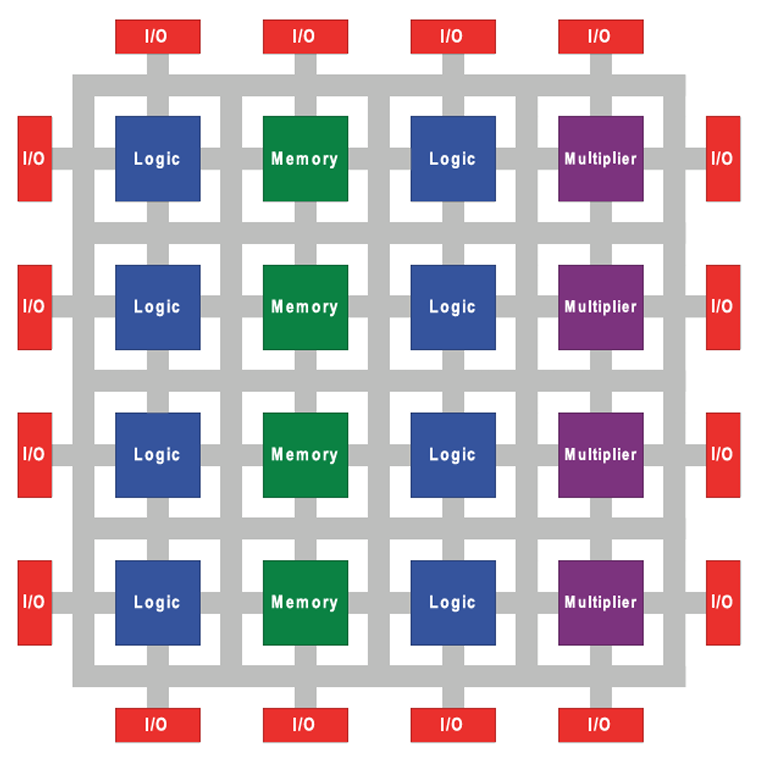
\includegraphics[width=0.6\linewidth]{pics/Uno.png} 
    \caption{Diagrama simplificado de matriz de programable de compuertas lógicas.}
    \label{fig:Uno}
    {\tiny Foundations and Trends in Electronic Design Automation (2008) 2 (2): 135--253. \url{https://doi.org/10.1561/1000000005}}
\end{figure}

\subsection{Tablas de búsqueda y elementos lógicos básicos}
Las tablas de búsqueda son la herramienta mediante la cual se genera la lógica en una FPGA, en lugar de utilizar compuertas lógicas y tener que redirigir miles de compuertas lógicas, lo que se utiliza son celdas de memoria en conjunto con multiplexores de esta manera se genera una tabla de verdad dentro del sistema mediante un flujo de bits que lo configura \cite{kuon2008fpga}. También son conocidas como LUTs, según la cantidad de entradas se le añade un número al final a modo de identificación, del número de entradas depende la cantidad de bits de configuración que tiene una tabla de búsqueda. Una LUT de k entradas almacena su tabla de verdad en $2^k$ bits de configuración. Una LUT4 requiere 16 bits y una LUT6 requiere 64. Aunque las tablas de búsqueda sean escalables es importante analizar las consecuencias de su escalabilidad, ya que existe una curva que describe los cambios en el área y cantidad de tablas de búsqueda en cierta área \cite{kuon2008fpga}.

\begin{figure}[h!]
    \centering 
    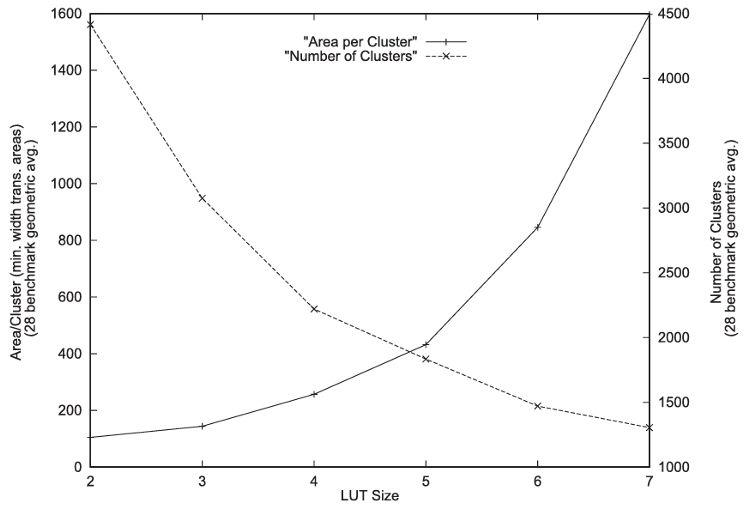
\includegraphics[width=0.7\linewidth]{pics/Dos.png} 
    \caption{Grafica de LUT de uso optimo.}
    \label{fig:Dos}
    {\tiny Foundations and Trends in Electronic Design Automation (2008) 2 (2): 135--253. \url{https://doi.org/10.1561/1000000005}}
\end{figure}

En la Figura \ref{fig:Dos} se muestra que el punto óptimo del tamaño de las tablas de búsqueda se encuentra cerca de LUT5, no obstante, se aclara que esto no impide tener LUT6 aunque solo se cuente con LUT5, debido a que se va a trabajar con conglomerados de LUTs estos se pueden conectar en paralelo para crear tablas de búsqueda modulares que representen un LUT6, a forma de ejemplo los LUT5 tienen 32 posiciones de memoria y los LUT6 tienen 64 posiciones de memoria, por lo que al utilizar dos LUT5 se puede generar la lógica necesaria para un LUT6 \cite{kuon2008fpga}. La práctica anterior es una eficiente solución para evitar el malgasto de área de la FPGA en tablas de búsqueda. A nivel de implementación física se suele utilizar memoria estática de acceso aleatorio para las tablas de búsqueda y estos constituyen los bloques blandos de la FPGA \cite{kuon2008fpga}.

Se debe tomar en cuenta para la eficiencia de una FPGA, no solo tiene lógica reconfigurable, también cuenta con módulos especializados, en el caso de que toda la lógica sea reconfigurable, se pueden utilizar múltiples tablas de búsqueda en algo que no es necesario por ejemplo en bloques de multiplicación, este tipo de bloque es conocido como bloque rígido ya que su función es fija. Su implementación es grabada sobre el propio silicio haciéndola no reconfigurable, pero su ventaja se encuentra en su rendimiento ya que al estar sobre el silicio funcionan de manera más rápida que una tabla de consulta y requiere poca área del silicio \cite{kuon2008fpga}.

\subsection{Conglomerados lógicos}
En una FPGA el conglomerado lógico es el bloque básico y necesario, el conglomerado es un conjunto de tablas de búsqueda, la cantidad de tablas de búsqueda es definido por el arquitecto, sin embargo, hay un punto óptimo para el área del conglomerado y la cantidad de conglomerados según el tamaño de las tablas de búsqueda (Figura \ref{fig:Tres}), otro punto importante para la eficiencia del conglomerado es la manera de agrupar los bits de configuración de las SRAM del conglomerado \cite{F_kuon2005}.

\subsection{Red de interconexión} 
 La arquitectura del enrutamiento en una FPGA es lo que da conexión a las LUTs al igual que sus entradas, salidas y los bloques rígidos para completar la lógica diseñada. La arquitectura utilizada es la arquitectura tipo isla (Figura \ref{fig:Tres}) \cite{hassani2024efficient, kuon2008fpga, A_oliver2007}. En dicha arquitectura se tienen los bloques lógicos y canales de enrutamiento a los cuatro lados de dichos bloques lógicos, los números de pistas por canal se denominan ancho de canal W y se fija al diseñar la arquitectura, sin embargo, es de los parámetros más importantes que puede tener una FPGA ya que define la cantidad de señales que se pueden trabajar de manera simultánea \cite{hassani2024efficient, kuon2008fpga}.

\begin{figure}[h!]
    \centering 
    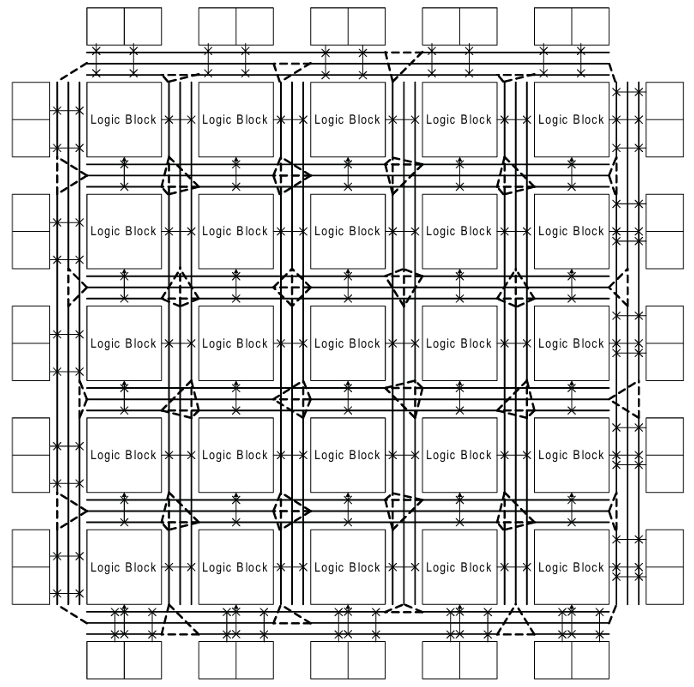
\includegraphics[width=0.6\linewidth]{pics/Tres.png} 
    \caption{Diagrama de configuración del enrutamiento y bloques lógicos.}
    \label{fig:Tres}
    {\tiny Foundations and Trends in Electronic Design Automation (2008) 2 (2): 135--253. \url{https://doi.org/10.1561/1000000005}}
\end{figure}


La lógica de la arquitectura de isla se basa en dos sencillos términos, cables largos y cables cortos, los cables largos componen los canales que se observan en paralelo a los bloques lógicos, su principal función es ser una malla de interconexión entre las señales que se generen o ingresen a la FPGA \cite{hassani2024efficient, kuon2008fpga}. Los cables cortos son el medio por el que las señales entran a un bloque desde la malla de enrutamiento o por la que la señal sale de un bloque a la malla de enrutamiento (Figura \ref{fig:Cuatro}) \cite{kuon2008fpga}.

\begin{figure}[h!]
    \centering 
    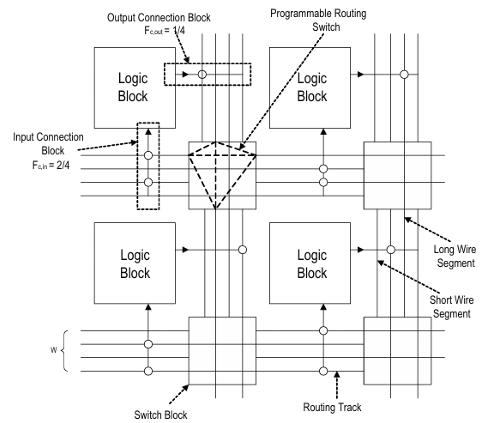
\includegraphics[width=0.6\linewidth]{pics/Cuatro.png} 
    \caption{Diagrama de bloques de cables cortos y largos.}
    \label{fig:Cuatro}
    {\tiny Foundations and Trends in Electronic Design Automation (2008) 2 (2): 135--253. \url{https://doi.org/10.1561/1000000005}}
\end{figure}


Cabe mencionar que existen arquitecturas de enrutamiento que dependen del orden jerárquico para ordenar la transferencia de datos, pero a manera que la jerarquía aumenta, los retardos aumentan de manera significativa, perdiendo el sentido de que existan múltiples niveles jerárquicos y haciendo esta arquitectura contraproducente al objetivo de flexibilidad inherente de una FPGA \cite{kuon2008fpga}. La malla de enrutamiento se encarga del desplazamiento de datos en la arquitectura de una FPGA, no obstante, la gestión de los datos es responsabilidad de la matriz de conmutación \cite{hassani2024efficient, kuon2008fpga}.

La malla de enrutamiento conecta todos los bloques de la arquitectura, pero aún se deben dirigir dichos datos, para que sean la entrada de un bloque o inclusive para que dos bloques trabajen los datos en paralelo, la matriz de conmutación es el mecanismo mediante el cual se ordenan las pistas de cables y se define a las señales cuál bloque es su próximo ingreso \cite{kuon2008fpga}. Estas rutas se definen desde que se carga el flujo de bits a la FPGA, por lo que las rutas son flexibles previas al flujo de bits, pero estáticas una vez programadas. Su funcionamiento se caracteriza por el uso de multiplexores para definir la ruta, sin embargo, también se implementa la lógica necesaria mediante transistores de paso para definir su ruta \cite{hassani2024efficient}.

Se considera la intersección de dos canales como una matriz de conmutación, en dichos canales donde cada cable interseca con otro cable se debe considerar la posibilidad de que la señal viaje sobre el mismo cable en la misma dirección inicial, que siga una ruta ascendente por el cable con el que interseca, o una ruta descendente por el cable que interseca. Para definir la ruta específica que se desea, se requieren de al menos seis transistores de paso para aislar la ruta en el caso de que no se desee bifurcar la señal, las ubicaciones específicas para dichos transistores de paso son conectando la sección de cable izquierdo con el derecho, conectando la sección ascendente con la descendente, la izquierda con la ascendente, la izquierda con la descendente, la ascendente con la derecha y la descendente con la derecha, de esta manera se tiene un control total sobre la dirección deseada de la señal, su control se basa en los datos guardados en una memoria estática de acceso aleatorio que requiere seis bits de control, considerando un bit por transistor de paso y una memoria estática de acceso aleatorio por intersección de los cables largos tal (Figura \ref{fig:Cinco}) \cite{kuon2008fpga}.

\begin{figure}[h!]
    \centering 
    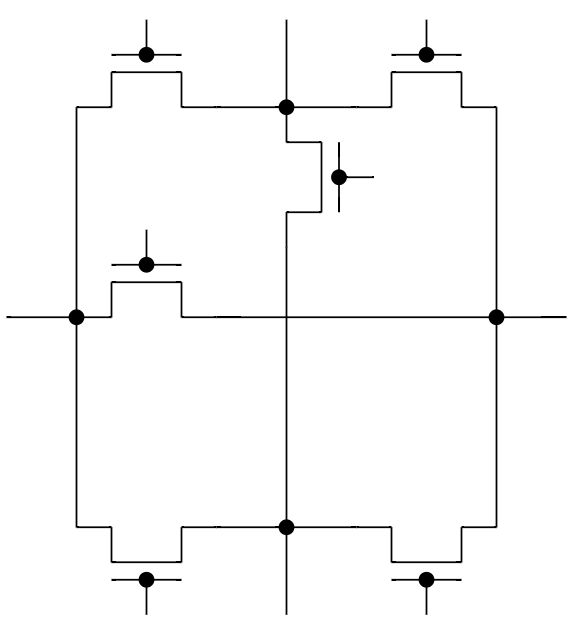
\includegraphics[width=0.4\linewidth]{pics/Cinco.png} 
    \caption{Diagrama matriz de conmutación.}
    \label{fig:Cinco}
    {\tiny Foundations and Trends in Electronic Design Automation (2008) 2 (2): 135--253. \url{https://doi.org/10.1561/1000000005}}
\end{figure}


\section{FABulous}
\subsection{Definición del fabric mediante azulejos}
La unidad básica del fabric o arquitectura, son los “tiles” que se traducen a azulejos. Se puede considerar a la arquitectura de la FPGA como un mosaico de azulejos, se disponen columnas del mismo tipo de bloque para formar una matriz que será utilizado posterior a la configuración \cite{G_koch2021}. Existen múltiples tipos de azulejos, los más comunes son LUT, multiplicador DSP, RegFile y Ram\_IO, su función varia y no hay obligación de que la arquitectura cuente con todos los tipos de azulejos \cite{G_koch2021}.

\subsection{Azulejos de FABulous utilizados en este trabajo}
En la subsección anterior se explica que es un azulejo y como su funcionalidad depende de si es una LUT, multiplicador DSP, RegFile o Ram\_IO, se debe profundizar en el funcionamiento individual de cada uno de estos bloques para entender la esencia del comportamiento de FABulous \cite{fabulous2024, meschkov2025design}. El azulejo LUT como se explico anteriormente es la tabla de búsqueda que busca emular comportamientos aritméticos o lógicos. El multiplicador DSP es un tipo de bloque duro, esto significa que no es reconfigurable y están hechos con una operación especifica para no sobre utilizar tablas de búsqueda, en este caso la multiplicación \cite{fabulous2024}. Los azulejos DSP están hechos para que haya un uso eficiente de los recursos, el inconveniente que puede presentar su uso es que son azulejos del doble de grande de un azulejo estándar \cite{H_bottcher2023}. El azulejo RegFile es un banco de registros pequeño con un puerto de escritura y varios puertos de lectura \cite{fabulous2024}. Los azulejos RAM\_IO hacen la conexión entre la memoria de acceso aleatoria de la FPGA, las entradas y las salidas, para optimizar la comunicación \cite{G_koch2021}.

\section{Flujo de implementación para FPGAs}
\subsection{Síntesis lógica y mapeo tecnológico}
La finalidad de la síntesis lógica es determinar las compuertas a utilizar por el diseño, por lo tanto, se genera una construcción estructural a nivel lógico \cite{N_lopezvallejo2004, K_maldonado2011}. Su principio es la traducción del lenguaje de descripción de hardware a las compuertas básicas que son necesarias para implementar dispositivo bajo prueba \cite{I_demicheli2005}. Una herramienta de código abierto que permite la síntesis lógica de un diseño de manera efectiva es Yosys, que trabaja en conjunto a FABulous, para implementar un diseño dentro de la FPGA diseñada mediantes FABulous \cite{wolf2024yosys, fabulous2024}.

\subsection{Generación del flujo de bits}
El flujo de bits, también llamada bitstream, es la cadena de valores lógicos altos y bajos con los que se configura la FPGA, anteriormente se habia descrito de manera breve, pero la profundidad del proyecto merece que el tema sea descrito en detalle. Se aclara que la literatura utilizada para esta sección hace referencia principalmente a las FPGAs de Xilinx, al ser propietarios el comportamiento puede variar, pero en un macro contexto todas las FPGAs funcionan de manera similar \cite{shan2019fpga, M_terasic2017, L_altera2025}.

La sucesión para llegar al flujo de bits inicia por netlist que Yosys genera durante la síntesis lógica, nextpnr coloca, enruta y escribe un archivo FASM, FABulous traduce el archivo FASM a bits según la especificación de la arquitectura, organizados en tramas. Este escenario es utilizado para comprender el uso del diseño con respecto a lo disponible en la FPGA \cite{J_note2008}. El flujo de bits solo contiene lo necesario para la configuración de la lógica interna de la FPGA, por lo que datos como nombres de cables o nodos son desperdicios de los archivos anteriores a la generación de bits que no son irrelevantes para conocer el estado del diseño y la FPGA, pero si para la configuración y por lo tanto no pasan a la siguiente etapa \cite{J_note2008, shan2019fpga}.

El problema del flujo de bits propietarios, se encuentran cifrados y eso aumenta el tiempo de configuración considerablemente, de igual manera deja de tener un comportamiento determinista por lo que realizarle cambios al flujo de bits manualmente no necesariamente se puede observar cómo afectan dichas variantes \cite{J_note2008}. La estructura del flujo de bits pasa a una maquina de estados que inicialmente discrimina el marco de configuración del resto de bits, esto a su vez permite que se comprenda la secuencia de bits y se construye un arreglo con el resto de bits dividiéndolo en múltiples marcos de configuración indexados listos para su distribución por la FPGA, la mayoría de los bits son utilizados para la configuración de ruteo e interconexiones y el resto para la lógica \cite{J_note2008}. 

\section{Configuración mediante JTAG}
Considerando el funcionamiento de una FPGA, es necesario tener un conocimiento del proceso entre el diseño y la descripción de hardware, para cualquier sistema, esto debido al flujo de bits necesario para dar propósito a la FPGA. Se debe implementar un inyector del flujo de bits además de la FPGA embebida en el nivel superior de jerarquía, de otra manera la FPGA embebida se mantiene en un estado sin programar \cite{nelsonBoundaryScan, xjtagWhatIsJtag}. Se requiere algún tipo de memoria que se pueda utilizar para luego serializar y cargarla a la FPGA embebida. Las memorias de solo lectura cumplen con características específicas para probar el funcionamiento de la FPGA   embebida en conjunto con lógica secuencial que permite la serialización de los datos de la memoria de solo lectura para su posterior inyección en el sistema, de esta implementación suele encargarse el software de diseño en conjunto con los puertos del hardware para la configuración \cite{ieee1149, nelsonBoundaryScan}.

El Joint Test Action Group, fue desarrollado para resolver problemas en el área de prueba de circuitos integrados, esto debido a que los circuitos integrados cada vez disminuían el tamaño y los pines de prueba que se utilizaban acaparaban mucha área del circuito integrado por lo que se investigaban nuevos métodos de probar la funcionalidad de los circuitos integrados \cite{ieee1149}. El estándar IEEE 1149.1 surge en 1990 y define la arquitectura TAP en conjunto con el JTAG para diagnóstico, manufactura, validación, caracterización y debug de los circuitos integrados \cite{ieee1149}. 

\begin{figure}[h!]
    \centering 
    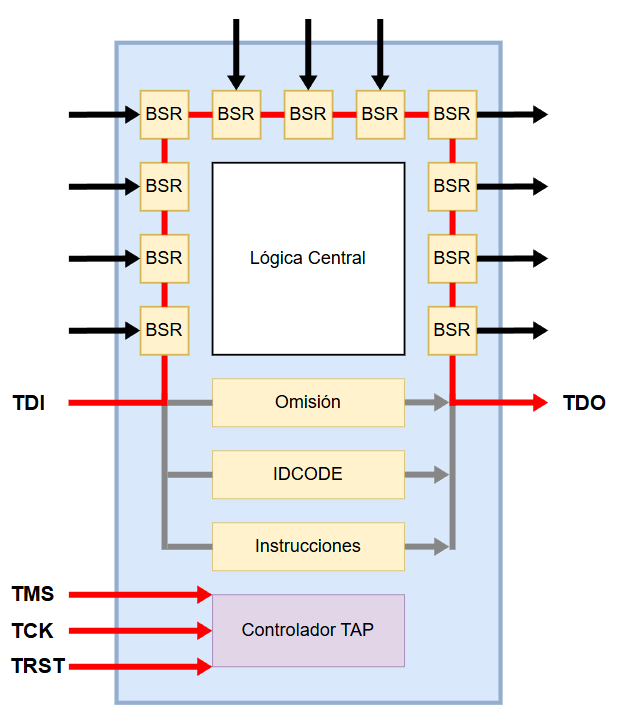
\includegraphics[width=0.4\linewidth]{pics/Seis.png} 
    \caption{Diagrama de la arquitectura TAP.}
    \label{fig:Seis}
    {\tiny JTag Boundary Scan. \url{https://www.jtag.com/boundary-scan/}}
\end{figure}


La conexión física se basa en 4 pines, TDI (Entrada de datos serial), TMS (Control), TCK (Reloj), TDO (Salida de datos serial) y en ocasiones se añade un pin extra TRST (Reinicio asincrónico), estas cuatro o cinco señales son conocidas como TAP (Puertos de acceso para pruebas). En el contexto de las FPGAs, se utiliza el JTAG para acceder a la configuración de la memoria para programar el dispositivo, para visualizar la lógica programable del núcleo y el ruteo de los recursos. Esto se ejemplifica en las secciones pasadas dedicadas a explicar la arquitectura de lógica reconfigurable de las FPGAs, donde los registros SRAM configuran las tablas de consulta, los caminos que deben seguir los recursos y la disposición de las matrices de conmutación \cite{jtagTechnologiesBoundaryScan, ieee1149}.

\begin{figure}[h!]
    \centering 
    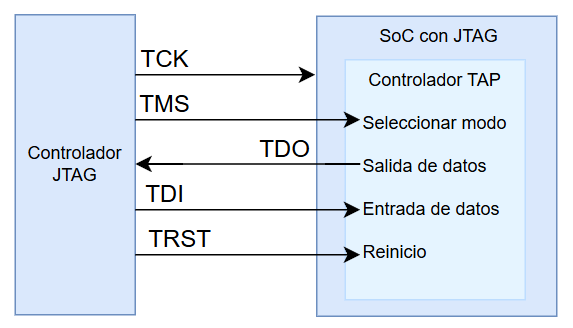
\includegraphics[width=0.6\linewidth]{pics/Siete.png} 
    \caption{Diagrama de conexion JTAG y TAP.}
    \label{fig:Siete}
    {\tiny How the {JTAG} {TAP} Controller Works. \url{https://www.jtag.com/how-the-jtag-tap-controller-works/}}
\end{figure}


\subsection{Máquina de estados del controlador TAP}
El controlador TAP es el mecanismo de control base del estándar IEEE 1149.1, en este se define como los datos son ciclados a través del dispositivo y determina si se accede a alguno de los registros de datos e/o instrucciones \cite{jtagTechnologiesTapController, ieee1149}. Las señales del controlador se acceden mediante la interfaz TAP explicada anteriormente. El pin de mayor significado para el controlador TAP es el TMS debido a que es la entrada de la máquina de estados que define el camino a tomar de los 16 estados existentes \cite{jtagTechnologiesTapController}. Hay tres funcionalidades que ejecuta la máquina de estados, el estado de prueba de lógica de reinicio y marcha/inactivo, el estado de acceso al registro de instrucciones (IR) y el estado de acceso a los registros de datos (DR) \cite{jtagTechnologiesTapController}.

\begin{figure}[h!]
    \centering 
    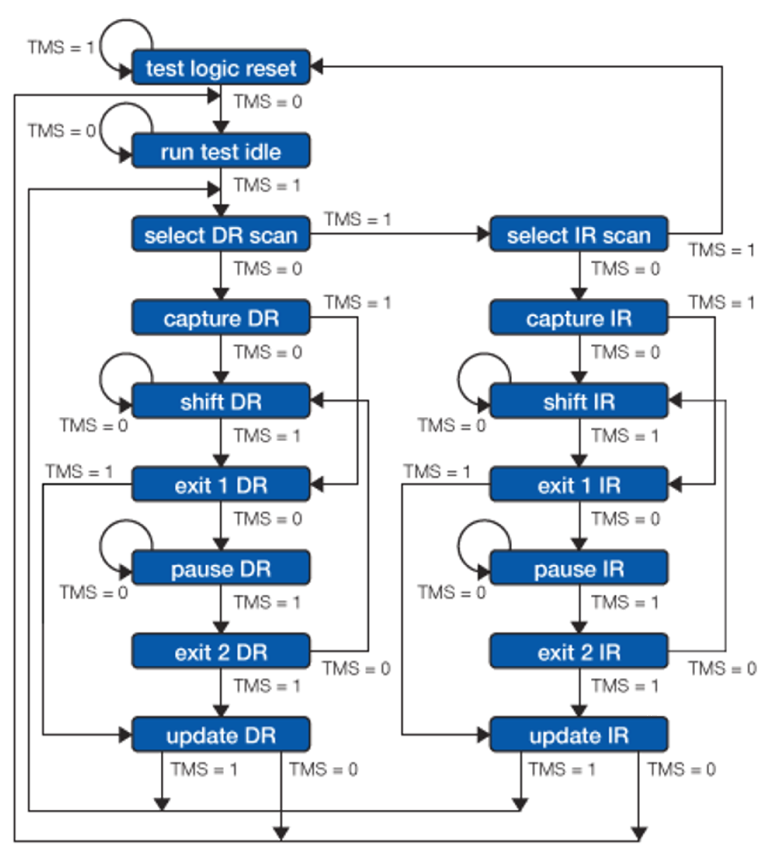
\includegraphics[width=0.6\linewidth]{pics/Ocho.png} 
    \caption{Máquina de estados del controlador TAP.}
    \label{fig:Ocho}
    {\tiny How the {JTAG} {TAP} Controller Works. \url{https://www.jtag.com/how-the-jtag-tap-controller-works/}}
\end{figure}

\subsection{Registros de instrucción y de datos}
El estándar IEEE 1149.1 define dos tipos de registros, los registros de datos y los registros de instrucciones. Los registros de datos incluyen el registro de escaneo de frontera (BSR), el registro de omisión (BYPASS) y el registro del código de identificación (IDCODE) \cite{jtagTechnologiesTapController, ieee1149}. El controlador TAP se encarga de definir a cuál se lee mediante la máquina de estados ya que solo se puede utilizar un registro de datos a la vez. 

El BSR no es un registro de un solo bloque, sino en una cadena de bloques que funcionan como registro de corrimiento para forzar valores a pines específicos internamente en el SoC, de igual manera se puede utilizar como un muestreo de los valores de los pines considerando que son solo de lectura para realizar un censado \cite{jtagTechnologiesTapController, ieee1149}. El registro de omisión solo cuenta con un bit de longitud, y su función es habilitar o desconectar el uso del registro BSR, funciona como paso a la entrada de otros SoC que se quieren probar en serie con el primero, esto permite la optimización del flujo de bits. El registro del código de identificación es un registro de 32 bits que contiene la identificación única del dispositivo, está grabada en el silicio para evitar su modificación, sirve para que el software sea capaz de identificar el hardware y el usuario utilice valores correctos de tensión para el registro BSR y la correcta cantidad de bits \cite{jtagTechnologiesTapController, ieee1149}.

\section{Fundamentos de los circuitos de prueba}
\subsection{Filtros de respuesta finita al impulso}
Un filtro FIR calcula cada muestra de salida como la suma ponderada de la muestra actual y de un número finito de muestras anteriores de la entrada, lo que corresponde a una convolución entre la señal y la respuesta al impulso del filtro \cite{proakis1996digital}. Matemáticamente se puede explicar secuencialmente como un desplazamiento temporal, la multiplicación de la señal por otra señal de referencia y la suma de los resultados para generar el muestreo de la salida \cite{meyerbaese2014digital, proakis1996digital}. Los filtros digitales de respuesta finita al impulso como su nombre lo indica tienen una respuesta finita al impulso, esto significa que su salida se vuelve cero después de un número finito de muestras \cite{meyerbaese2014digital, proakis1996digital}. Al no tener realimentación, los filtros FIR son siempre estables. Tienen fase lineal cuando sus coeficientes son simétricos o antisimétricos \cite{proakis1996digital} 

\subsection{Multiplicación de matrices}
El producto de dos matrices solo se define cuando el número de columnas de la primera coincide con el número de filas de la segunda. Si A es de orden mxn y B es de orden nxp, el producto AB es una matriz de orden mxp \cite{O_mayhua2018}. Cada elemento cij de la matriz resultado se obtiene sumando los productos de los elementos de la fila i de A por los elementos correspondientes de la columna j de B, de modo que cij = ai1 b1j + ai2 b2j + ... + ain bnj \cite{O_mayhua2018}. El producto de matrices no es conmutativo, de manera que en general AB y BA son matrices distintas \cite{O_mayhua2018}.

\section{FPGAs embebidas comerciales}
Las FPGAs se utilizan como solución antes piezas de hardware caras cuyo diseño no es complejo a nivel de características como la potencia requerida o almacenamiento significativo \cite{saidi2020survey}. Su uso se encuentra incluso vinculado a ASICs ya que también significa ahorro para los productores de dicho ASIC, no obstante, en casos de eFPGAs en ASICs, las eFPGAs cuentan con características específicas para la pieza de hardware que se desea implementar en conjunto con el ASIC, por lo que no se espera una gran cantidad de tablas de consulta, menores velocidades de reloj para lógica secuencial, e incluso puede que no se cuente con bloques rígidos especializados a menos que el ASIC lo requiera \cite{saidi2020survey}. 

Flex Logic es una compañía tecnológica que utiliza la tecnología de eFPGA desde el 2015, los motiva la reutilización de un circuito integrado luego de su fabricación \cite{saidi2020survey}. Cuentan con un núcleo de eFPGA conocido como FLX10 con cinco a siete capas de metal, sus características principales son veinte mil bits de memoria de acceso aleatorio, aproximadamente ciento veintidós mil quinientos tablas de búsqueda de seis entradas y pueden incluir grano grueso \cite{saidi2020survey}.

Menta trabaja con eFPGA desde el 2009, al igual que Flex Logic su objetivo es la modificación de hardware post producción \cite{saidi2020survey, abderrahmaneMaximizeFlexibility}. La eFPGA de Menta cuenta con sus propias herramientas para la compilación, diseño en RTL y configuración del eFPGA llamada Origami. Cuenta con aproximadamente doscientos mil tablas de búsqueda de cuatro entradas y es de grano fino \cite{saidi2020survey, abderrahmaneMaximizeFlexibility}.

Achronix trabaja con eFPGA desde el 2016 su modelo de Speedcore eFPGA incluye bloques de RAM, y bloques de procesamiento de señales digitales. Cuenta con el software ACE para el diseño de herramientas, su principal uso es como acelerador de hardware y coprocesador reconfigurable, tiene aproximadamente mil tablas de búsqueda y pueden incluir grano grueso \cite{abderrahmaneMaximizeFlexibility}.

NanoXplore es una compañía que data del 2014 cuenta con la eFPGA NX-eFPGA que se puede configurar mediante la aplicación NanoXmap para sintetizar RTL hasta el flujo de bits, el uso de tablas de consulta de cuatro entradas le permite utilizar menor área para la eFPGA en la ASIC predeterminada, incluye aproximadamente setecientos cincuenta mil tablas de búsqueda y pueden incluir grano grueso \cite{abderrahmaneMaximizeFlexibility}.

La academia también presenta varias arquitecturas de eFPGA entre ellas la FASE eFPGA, EFPGA Based on Multistage Switching Networks, ACLBs eFPGA, Overlay eFPGA, EFPGAs based on a flexible architecture, ESL Re-programmable eFPGA, EFPGA Subsystem, LIP6 eFPGA y FlexTiles, no se detallan sus características debido a que la mayoría utiliza tablas de búsqueda de entre cuatro y seis entradas. Su uso es similar, sustituir una ASIC costosa en la implementación de un proyecto o para investigación de su desarrollo \cite{saidi2020survey, abderrahmaneMaximizeFlexibility}.

En el ámbito de las eFPGA implementadas en ASICs, se observa la predominación de la utilización de tablas de consulta de cuatro, cinco y seis entradas \cite{saidi2020survey, abderrahmaneMaximizeFlexibility}. Esta selección no es arbitraria, sino el resultado de una optimización que busca el equilibrio óptimo entre el área del conglomerado lógico, la densidad de los conglomerados y la complejidad interna de cada tabla de búsqueda \cite{saidi2020survey, abderrahmaneMaximizeFlexibility}.

La elección del número de entradas en una tabla de búsqueda conlleva un compromiso entre la cantidad de entradas y su área, debido a que el incremento en el número de entradas permite implementar funciones lógicas más complejas con menor cantidad de niveles de lógica, reduciendo los retardos de propagación, este incremento aumenta simultáneamente la superficie del conglomerado y la carga capacitiva interna. En consecuencia, el diseño de una arquitectura eficiente requiere una correlación precisa entre estas variables para maximizar la eficiencia de área, definida como el área total del conglomerado normalizada por su capacidad de procesamiento, garantizando que el diseño final sea tanto eficaz en términos de velocidad como compacto en términos de ocupación de silicio \cite{saidi2020survey, abderrahmaneMaximizeFlexibility}.

Se observa el uso de una granularidad gruesa, la cual se diferencia de las arquitecturas de grano fino al optimizar el procesamiento de palabras de datos completas en lugar de realizar operaciones bit a bit \cite{saidi2020survey, abderrahmaneMaximizeFlexibility}. Esta preferencia responde a la necesidad de eficiencia en el rendimiento debido a que, al operar sobre vectores de datos de mayor longitud, se logra reducir el número de ciclos de reloj necesarios para completar operaciones complejas, como multiplicaciones o registros de desplazamiento \cite{saidi2020survey, abderrahmaneMaximizeFlexibility}.

La preferencia hacia el grano grueso permite abstraer la funcionalidad lógica a niveles superiores, lo que mejora la velocidad de ejecución, lo que también simplifica la interconexión entre conglomerados \cite{saidi2020survey, abderrahmaneMaximizeFlexibility}. En comparación, una arquitectura de grano fino, aunque es versátil para manipular señales a nivel de bit, se vuelve ineficiente en términos de retardo de propagación y consumo de recursos \cite{saidi2020survey, abderrahmaneMaximizeFlexibility}.


%%%%%%%%%%%%%%%%%
\chapter{Prueba de concepto}
\label{ch:diseño}

\section{Ambiente de simulación de código abierto}

Se instaló Linux como un subsistema de Windows, lo que permite ejecutar un entorno Linux directamente dentro de Windows, sin necesidad de usar una máquina virtual ni hacer un arranque dual. Se eligió el WSL debido a su facilidad de uso, la comodidad al momento de acceder a los archivos de síntesis y la simplicidad de transferir archivos al sistema operativo por defecto del computador. Además, al correr sobre el mismo equipo, el ambiente de simulación comparte recursos con Windows, lo que permite utilizar las herramientas de código abierto sin dedicar una máquina exclusiva para ello. El uso de un ambiente UNIX era necesario para cumplir con el objetivo del proyecto de simular mediante código abierto, ya que varias de las herramientas principalmente utilizadas solo corren en distribuciones de Linux. La elección de la distribución específica de Linux se puede considerar fortuita. No obstante, existía experiencia previa y reciente con Ubuntu. No hay gran diferencia entre las distribuciones, pero por la razón anteriormente mencionada se utilizó la consola de Ubuntu 26.04 LTS.

El ambiente se compone de múltiples herramientas, y las prioritariamente necesarias son: Python, FABulous, Yosys, Nextpnr e Iverilog. Son necesarias debido al componente del flujo de trabajo que representan. El flujo de trabajo inicia con FABulous, mediante la creación del fabric.csv, que describe la configuración de la arquitectura seleccionada, utilizando los distintos “azulejos” para armar la arquitectura de isla deseada. Python es el lenguaje sobre el cual funciona FABulous y se utiliza también para los scripts de automatización del flujo. Nextpnr permite que un diseño sea simulado en la FPGA mediante el ruteo de los datos y el flujo de bits que el mismo Python provee del ruteo de nextpnr como un archivo binario. El análisis y la síntesis de los circuitos de prueba se realizan mediante Yosys, que posteriormente también es quien compila el diseño en conjunto con la FPGA generada. Por su parte, Iverilog es el simulador que permite ejecutar el testbench y verificar el comportamiento del sistema completo antes de llevarlo a hardware. En el caso presente, como se desea probar en una FPGA física, se incluyó en el circuito de prueba el JTAG necesario, en conjunto con una memoria de solo lectura que almacena el flujo de bits para su inyección posterior en el fabric.

Al flujo descrito (ver Figura 3.1) se le debe añadir un script para convertir el flujo de bits de un archivo binario a un archivo hexadecimal. Este es el formato requerido para inicializar la memoria de solo lectura en el diseño. Además de esto, se comprobó el funcionamiento de la FPGA en conjunto con el circuito de prueba mediante un testbench que incluye el sistema completo, flujo de bits incluido, y que da como realimentación una bandera de fallo o paso. La prueba funcional realizada incluye dos pruebas concretas: control positivo y control negativo. El control positivo se realiza con el total del flujo de bits para revisar que el JTAG esté cargando de manera satisfactoria el flujo de bits y que el circuito de pruebas se comporte como se espera. En este caso, la bandera esperada es la de paso. El control negativo carga parcialmente el flujo de bits. Su propósito es reconocer si en el control positivo hubo un falso positivo en el resultado del circuito de prueba con respecto al flujo de bits inyectado. Al estar el fabric configurado de forma incompleta, el circuito de prueba no debería producir la salida esperada, por lo que en este caso la bandera esperada es la de fallo. Si el control negativo también pasara, significaría que el testbench no es capaz de distinguir entre un fabric correctamente configurado y uno que no lo está, y por tanto el control positivo no sería confiable. Es importante aclarar que el resultado de estas banderas está vinculado con el testbench diseñado previamente y con el resultado esperado a la salida del circuito de prueba, por lo que se valida su funcionamiento.


%Imagen 1
\begin{figure}[h]
    \centering
    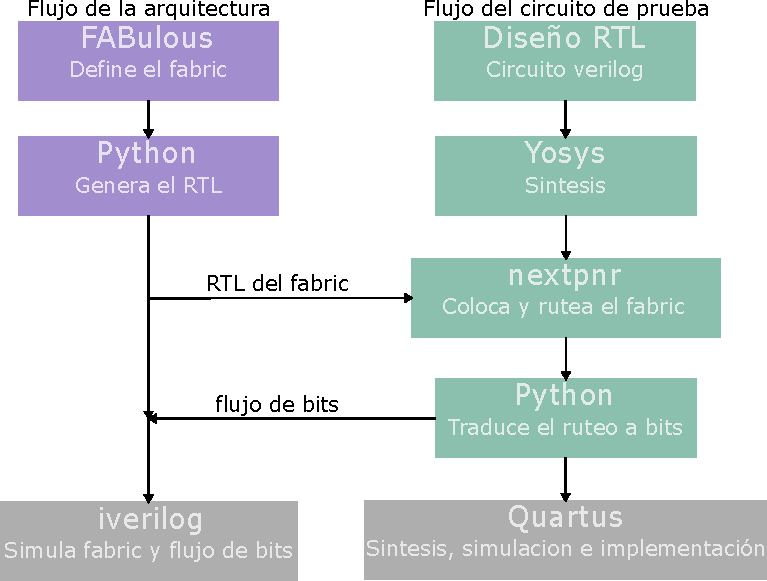
\includegraphics[width=0.8\textwidth]{../pics/diagFlujoAmb.pdf}
    \caption{Ambiente de simulación de código abierto}
    \label{fig:ambiente_simulacion}
\end{figure}

\section{Selección de las arquitecturas}

Se investigó el generador de FPGAs de FABulous. Anteriormente se menciona que funciona mediante azulejos. Sin embargo, existen catorce tipos de azulejos con los que se puede armar una FPGA, y el largo y ancho de la matriz para los azulejos no es constante, sino que se puede variar. Para tener una referencia se utilizó el fabric por defecto que FABulous ofrece y se comparó con dos arquitecturas encontradas en GitHub. No obstante, las dos arquitecturas habían sido generadas mediante el uso de FABulous. Al desconocer el propósito con el que se habían creado, ya que los repositorios estaban desactualizados y no incluían un README.md, se tomó la decisión de generar mediante FABulous las otras dos arquitecturas, variando los azulejos utilizados y el largo y ancho de la matriz. De esta manera se garantizó conocer con certeza la configuración de cada una y poder compararlas bajo las mismas condiciones.

De los catorce tipos de azulejos hay cinco funcionalidades diferentes. Los LUT4AB son el bloque lógico básico de las FPGA e incluyen un flip-flop para lógica secuencial y una cadena de acarreo, además de incorporar la matriz de direccionamiento para el ruteo de la FPGA. Los RegFile funcionan como un banco de registros pequeño con un puerto de escritura y varios puertos de lectura. Los azulejos DSP operan como un multiplicador o acumulador y, debido a su complejidad, tienen un tamaño mayor que el resto de azulejos. Por esta razón son los más adecuados para operaciones aritméticas intensivas, como las del multiplicador de matrices utilizado como circuito de prueba. Los RAM\_IO son azulejos que acceden a la memoria de acceso aleatorio del fabric y sirven para exponer los puertos de datos, dirección y control hacia dicha memoria. Los W\_IO son los azulejos que no tienen una función propia, pero sirven de entrada y salida para conectar los pines externos del chip con el fabric. En la matriz de azulejos se ubican en el borde oeste. El resto de azulejos son variantes de los recién explicados, y la diferencia recae en su ubicación en la matriz, ya sea al sur o al norte. Tienen el prefijo N\_term o S\_term para ordenar los cables de ruteo con respecto a la matriz. También existe la terminación single, que depende de si el azulejo tiene o no una columna adyacente del mismo tipo.

\section{Arquitecturas originalmente seleccionadas}

Como se mencionó anteriormente, la arquitectura 1 (ver Figura 3.2) es la configuración por defecto de FABulous, la cual incluía catorce filas sin incluir los terminadores y diez columnas, que se dividen en seis columnas de LUT4AB, una columna de RegFile, una columna de RAM\_IO, una columna de DSP y una columna de W\_IO. Esta arquitectura funciona como línea base, ya que las otras dos se definieron como variaciones de ella.

%Imagen 1
\begin{figure}[H]
    \centering
    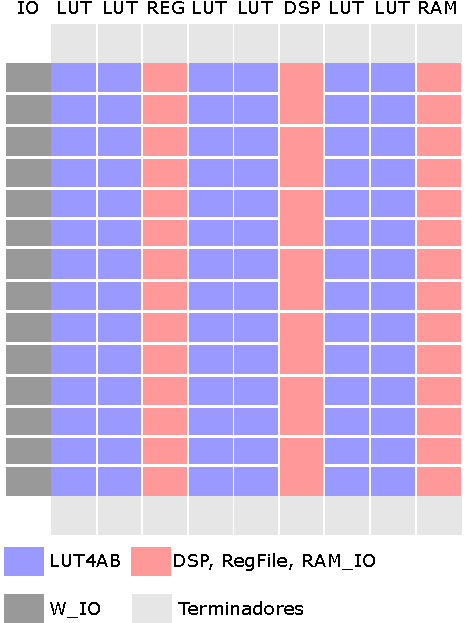
\includegraphics[width=0.5\textwidth]{../pics/Arq1.pdf}
    \caption{Arquitectura 1 - Configuración por defecto de FABulous}
    \label{fig:arq1}
\end{figure}

La arquitectura 2 (ver Figura 3.3) se configuró para contener el doble de azulejos DSP que la arquitectura 1. Originalmente esto se consideró en caso de que la arquitectura 1 fuera insuficiente para soportar el circuito de prueba del multiplicador de matrices con su JTAG y su memoria ROM para la inyección del flujo de bits. Por lo tanto, la arquitectura 2 incluía catorce filas sin contar los terminadores y diez columnas, de las cuales cinco se destinaron a LUT4AB, dos a DSP, una a RegFile, una a RAM\_IO y una a W\_IO. Cabe destacar que, para mantener el mismo número de columnas, la columna de DSP adicional se obtuvo a costo de una columna de LUT4AB, por lo que esta arquitectura cuenta con menos lógica de propósito general que la arquitectura 1.

%Imagen 1
\begin{figure}[]
    \centering
    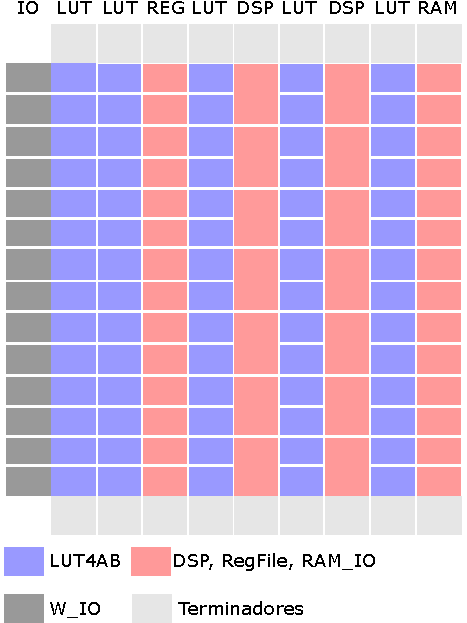
\includegraphics[width=0.5\textwidth]{../pics/Arq2.pdf}
    \caption{Arquitectura 2 - Variación con doble cantidad de azulejos DSP}
    \label{fig:arq2}
\end{figure}

La arquitectura 3 (ver Figura 3.4) es del doble de alta que la arquitectura 1. En este caso se quiso identificar si existía alguna consecuencia, a nivel de los parámetros medidos, según el tamaño del fabric, como por ejemplo retrasos mayores o mayor necesidad de potencia para su alimentación. Consiste de veintiocho filas sin contar los terminadores y diez columnas, entre ellas seis columnas de LUT4AB, una columna de RegFile, una columna de RAM\_IO, una columna de DSP y una columna de W\_IO. Al mantener la misma distribución de columnas que la arquitectura 1, la única variable que cambia es la altura, lo que permite atribuir cualquier diferencia en los resultados al tamaño del fabric y no a la composición de los azulejos.
\clearpage
\begin{figure}[H]
    \centering
    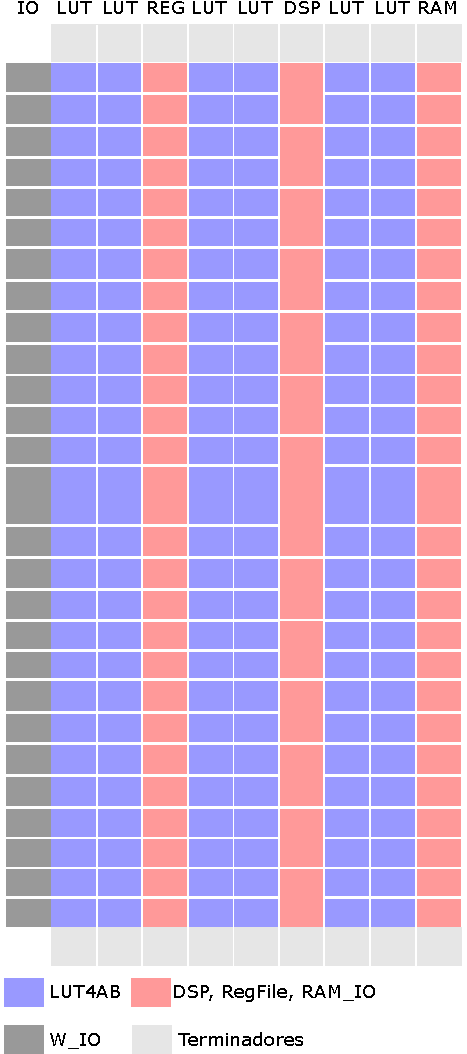
\includegraphics[width=0.5\textwidth]{../pics/Arq3.pdf}
    \caption{Arquitectura 3 - Variación con doble altura}
    \label{fig:arq3}
\end{figure}

\section{Circuitos de prueba originales}
\subsection{Filtro FIR}

Para evaluar las arquitecturas se utilizaron dos circuitos de prueba, un filtro FIR y un multiplicador de matrices. Ambos se describieron en Verilog con la misma interfaz de 28 pines de entrada y salida, por lo que se pudo utilizar el mismo top\_wrapper.v para los dos y cambiar únicamente la instancia del módulo.
El primer circuito es un filtro FIR pasa-bajos de cuatro etapas con coeficientes binomiales 1, 3, 3 y 1, divididos entre 8. Su ecuación es:

\[
    y[n] = (x[n] + 3x[n-1] + 3x[n-2] + x[n-3]) \gg 3
\]

El filtro no utiliza multiplicadores, ya que la multiplicación por tres se realiza sumando el dato consigo mismo desplazado un bit. Su ganancia es de uno en corriente directa y de cero en la frecuencia de Nyquist.

Las muestras de entrada son de 8 bits con signo. Internamente la suma se realiza con 11 bits para evitar desbordamientos, y el resultado se desplaza aritméticamente tres posiciones para obtener una salida de 8 bits. El filtro almacena las tres muestras anteriores en registros y solo procesa una muestra nueva cuando la señal valid está en alto. En ese caso, la señal y\_valid se activa durante un ciclo para indicar que la salida es válida.

\subsection{Multiplicador de matrices}

El segundo circuito multiplica dos matrices de 2x2 de enteros de 8 bits con signo, siguiendo la operación C = A x B. Utiliza un único multiplicador serie que trabaja por suma y desplazamiento. La salida requiere 17 bits con signo.

Los ocho elementos de entrada se cargan uno por ciclo en el orden A00, A01, A10, A11, B00, B01, B10 y B11. Al cargar el octavo elemento comienza el cálculo, durante el cual se ignora la señal load. Posteriormente salen los elementos C00, C01, C10 y C11, cada uno acompañado de la señal c\_valid durante un ciclo. 

\section{Traslado inicial del proyecto a Quartus®}

Una vez validado el funcionamiento del sistema en simulación, se procedió a trasladar el proyecto a Quartus\textregistered{} para probarlo en la tarjeta DE0-Nano-SoC de Altera\textregistered{}, la cual utiliza un Cyclone\textregistered{} V 5CSEMA4U23C6. En esta primera ocasión se incluyeron en el proyecto de Quartus\textregistered{} el fabric generado por FABulous, el circuito de prueba, el JTAG y la memoria de solo lectura con el flujo de bits. El objetivo era comprobar que el diseño completo podía sintetizarse e implementarse en la FPGA física.

Durante este intento se encontró que la FPGA embebida no cabía dentro de la FPGA de la tarjeta. Quartus\textregistered{} no logró completar la implementación del diseño debido a que se excedieron los recursos disponibles del dispositivo. El reporte de Quartus\textregistered{} indicaba que el diseño requería más LUTs y multiplexores de los disponibles en el Cyclone\textregistered{} V.

El resultado se debe a la naturaleza de una FPGA embebida. El fabric generado por FABulous se describe en Verilog, por lo que Quartus® lo trata como cualquier otro circuito y lo implementa con los recursos de la FPGA física. Esto significa que cada LUT, cada registro de configuración y cada multiplexor de las matrices de ruteo del fabric consume a su vez recursos lógicos del Cyclone® V. Una FPGA programable construida sobre otra FPGA es mucho más costosa en recursos que un diseño implementado directamente sobre la tarjeta. Sobre todo, el circuito de prueba, el JTAG y la memoria de solo lectura también compiten por los mismos recursos.

Este hallazgo determinó el rumbo del proyecto, ya que mostró que las arquitecturas y los circuitos de prueba definidos originalmente eran demasiado grandes para el dispositivo disponible. Como consecuencia, se decidió reducir tanto los circuitos de prueba como el tamaño de los fabrics, de manera que el sistema completo pudiera caber en la tarjeta.

\section{Arquitecturas reducidas}

Debido a que las arquitecturas originales no pudieron implementarse en la FPGA de la tarjeta, se generaron tres versiones reducidas de ellas, a las que se les llamó mini arquitecturas. Para cada una se conservó únicamente lo más distintivo de su arquitectura original, ya que el presupuesto de recursos del Cyclone\textregistered{} V no permitía más. Las primeras dos se diseñaron con 12 pines de entrada y salida disponibles para los circuitos de prueba, que también se redujeron en tamaño, mientras que la tercera se diseñó con 24 pines de entrada y salida. A continuación, se explica cada una por separado.

La mini arquitectura 1 (ver Figura 3.5) representa a la arquitectura 1, cuya característica distintiva es la columna de DSP. Consiste en seis filas sin contar los terminadores y cuatro columnas, que son una columna de W\_IO, dos columnas de LUT4AB y una columna de DSP. Su tamaño en Yosys fue de 10\,014 latches. Al ser la reducida de la arquitectura base, funciona como punto de referencia para comparar las otras dos.

%imagen 1 arqui mini 1
\begin{figure}[H]
    \centering
    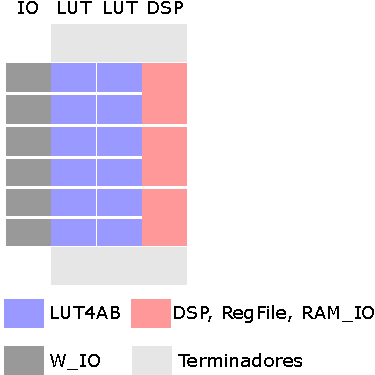
\includegraphics[width=0.5\textwidth]{../pics/ArqMini1.pdf}
    \caption{Arquitectura Reducida 1 - Configuración de referencia}
    \label{fig:arqmini1}
\end{figure}

La mini arquitectura 2 (ver Figura 3.6) representa a la arquitectura 2, que se distingue por tener el doble de DSP que la arquitectura 1. Mantiene las seis filas sin contar los terminadores, y tiene cinco columnas, que son una columna de W\_IO, dos columnas de LUT4AB y dos columnas de DSP. Su tamaño en Yosys fue de 12\,432 latches, el mayor de las tres. Esto es consecuencia directa de las columnas de DSP, que por su complejidad son los azulejos más grandes.

%imagen 1 arqui mini 2
\begin{figure}[H]
    \centering
    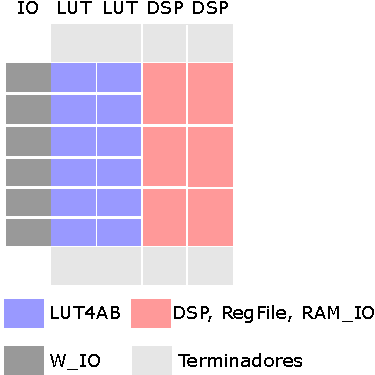
\includegraphics[width=0.5\textwidth]{../pics/ArqMini2.pdf}
    \caption{Arquitectura Reducida 2 - Configuración con doble cantidad de DSP}
    \label{fig:arqmini2}
\end{figure}

La mini arquitectura 3 (ver Figura 3.7) representa a la arquitectura 3, que se distingue por ser del doble de alta que la arquitectura 1. Por esta razón tiene doce filas sin contar los terminadores, el doble que las otras dos, pero solo dos columnas, que son una columna de W\_IO y una columna de LUT4AB. Su tamaño en Yosys fue de 7\,896 latches, el menor de las tres. Al tener el doble de filas de W\_IO, esta arquitectura cuenta con 24 pines de entrada y salida en el fabric. Los 12 pines de los circuitos de prueba se ubicaron en los pines 12 a 23, por lo que esta arquitectura además permitió comprobar que el circuito de prueba funcionaba con un desplazamiento de pines.

%imagen 1 arqui mini 3
\begin{figure}[H]
    \centering
    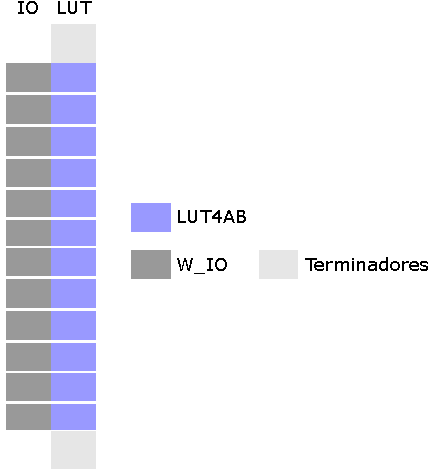
\includegraphics[width=0.5\textwidth]{../pics/ArqMini3.pdf}
    \caption{Arquitectura Reducida 3 - Configuración con doble altura}
    \label{fig:arqmini3}
\end{figure}

Las tres tienen la misma cantidad de lógica de propósito general, ya que las dos primeras tienen seis filas por dos columnas de LUT4AB y la tercera tiene doce filas por una columna. Esto permite comparar las geometrías sin que la capacidad lógica sea una variable adicional.

\section{Circuitos de prueba reducidos}

\subsection{Filtro FIR}

Una vez definidas las mini arquitecturas, fue necesario reducir también los circuitos de prueba para que entraran en ellas. Se conservaron las mismas dos funciones, el filtro FIR y el multiplicador de matrices, pero con datos de menor tamaño y con menos etapas. 
El FIR reducido es un filtro pasa-bajos de tres etapas con coeficientes 1, 6 y 1, divididos entre 8. Su ecuación es:

\[
    y[n] = (x[n] + 6x[n-1] + x[n-2]) \gg 3
\]

Las muestras de entrada y la salida son de 4 bits con signo. Los coeficientes caben en 4 bits con signo y su suma es 8, por lo que la ganancia en corriente directa es de uno y la salida cabe en 4 bits. Solo procesa una muestra cuando la señal valid está en alto y activa y\textunderscore valid durante un ciclo.

\subsection{Multiplicador de matrices}

El multiplicador reducido multiplica matrices de $2 \times 2$ con elementos de 2 bits con signo, es decir, con valores de menos 2 a 1. El resultado es de 5 bits con signo, con un rango de menos 16 a 15, ya que el mayor valor posible es 8. Conserva el mismo protocolo del multiplicador original. Se cargan ocho elementos en el orden A00, A01, A10, A11, B00, B01, B10 y B11, al octavo comienza el cálculo y salen C00, C01, C10 y C11, cada uno con c\textunderscore valid durante un ciclo. Utiliza un único multiplicador serie por suma y desplazamiento, que en este caso tarda dos ciclos por producto.

\section{Traslado final del proyecto a Quartus®}

Una vez validado el funcionamiento del sistema con los módulos reducidos en simulación, se procedió a trasladar el proyecto a Quartus®. Se realizó el proceso de análisis y síntesis, luego se compiló, se programó la tarjeta de la FPGA y se verificó el correcto funcionamiento mediante los LEDs y los conmutadores. Además de comprobar su funcionamiento, se generó el análisis de potencia. Ver Figura 3.8 para el diagrama de flujo del proyecto en Quartus®.

%imagen 1
\begin{figure}[H]
    \centering
    
\includegraphics[width=0.8\textwidth]{../pics/DiagQuartus.pdf}
    \caption{Diagrama de flujo del proyecto en Quartus®}
    \label{fig:diagquartus}
\end{figure}

Se creó un proyecto de Quartus\textregistered{} para cada combinación de arquitectura y circuito de prueba. Cada proyecto incluyó el módulo superior de la tarjeta, el \texttt{chip\_top}, la memoria de solo lectura con el flujo de bits, el módulo que envía el flujo de bits por el JTAG interno, el módulo JTAG propio y los archivos Verilog de los azulejos del fabric. No se incluyeron los archivos de FABulous destinados a la configuración externa, como la carga por UART y el modo bitbang, ni el archivo de la memoria RAM del fabric, ya que no eran necesarios y generaban errores durante la síntesis. La memoria de solo lectura se inicializó con el archivo hexadecimal correspondiente a cada arquitectura y circuito de prueba. Los pines de la tarjeta se asignaron a partir del archivo de asignaciones del fabricante, del cual se derivó un archivo con únicamente los pines utilizados. Además, se agregó un archivo de restricciones de tiempo.

Para la configuración de la arquitectura de FPGA embebida dentro de la placa DE0-Nano-SoC se consideró necesario implementar un módulo JTAG interno que operara de manera independiente al JTAG propio de la placa. Su funcionamiento requirió una memoria de solo lectura, una ROM, previamente cargada con el flujo de bits específico de la implementación del circuito de prueba correspondiente, ver Figura \ref{fig:diagUltimo}. Así, el JTAG interno tiene como función principal cargar de forma serial el flujo de bits almacenado en la memoria hacia la FPGA embebida para su configuración. Es importante diferenciar el JTAG del Cyclone V del JTAG interno. El JTAG del Cyclone V es un módulo físicamente ubicado en la placa y es el encargado de configurar la FPGA para las implementaciones. En cambio, el JTAG interno es un módulo implementado en la lógica de la propia FPGA Cyclone V.

\begin{figure}[H]
    \centering
    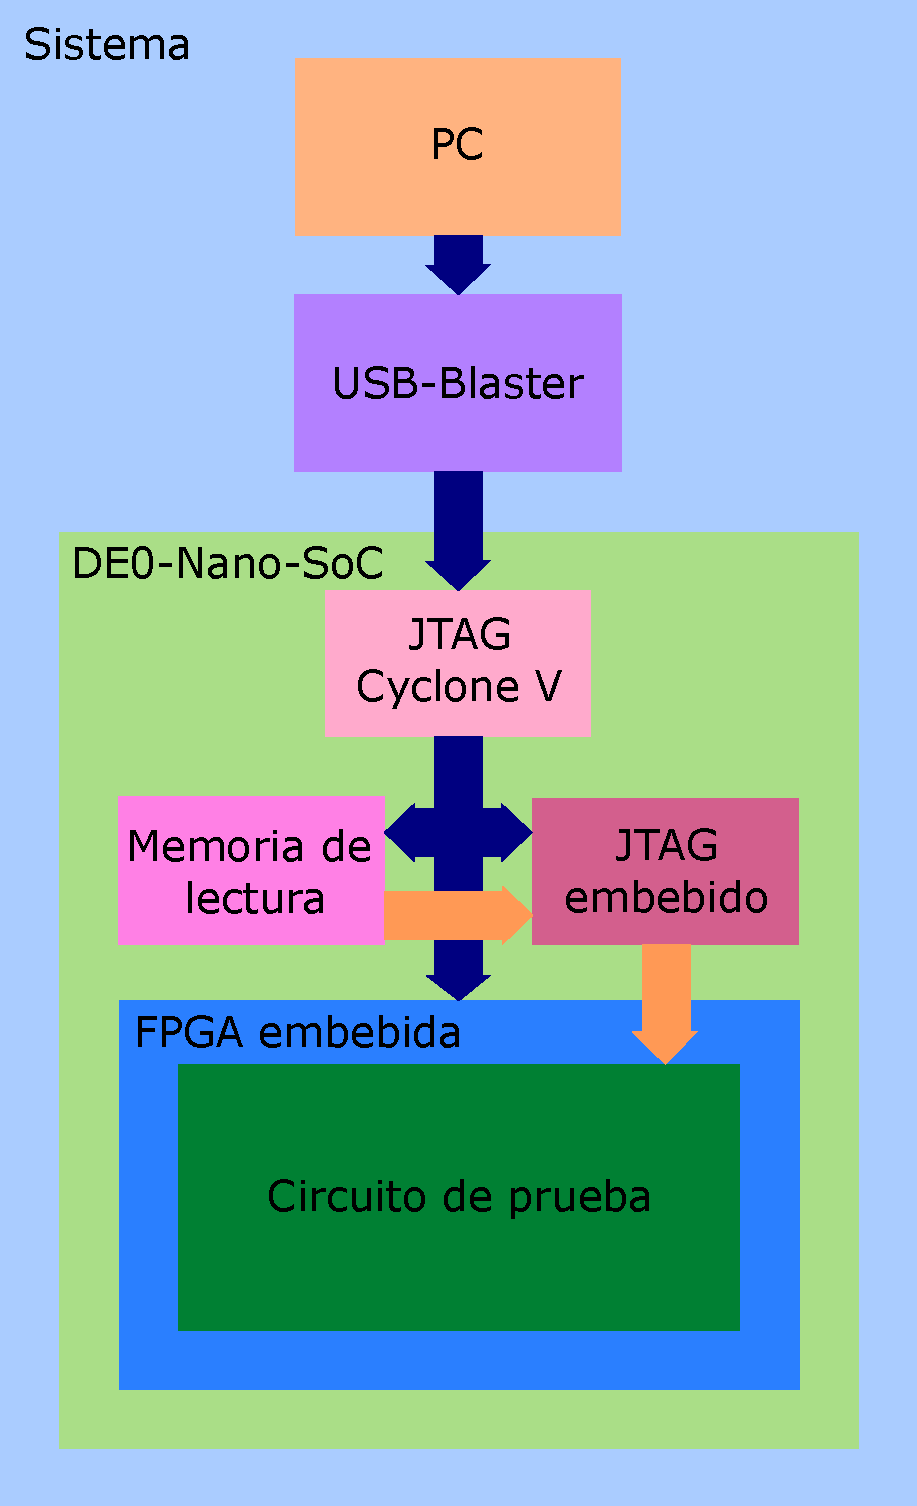
\includegraphics[width=0.4\textwidth]{../pics/diagUltimo.pdf}
    \caption{Diagrama de bloques del proyecto}
    \label{fig:diagUltimo}
\end{figure}

Durante la primera programación de la tarjeta se presentó un problema con la asignación de los pines. Al realizar la síntesis y la compilación, el diseño se implementaba sin que los puertos del módulo superior quedaran ubicados en los pines físicos de la FPGA. Como consecuencia, los LEDs permanecían en un estado fijo y los conmutadores no tenían ningún efecto sobre el diseño. Al revisar el Pin Planner se comprobó que ninguno de los puertos tenía un valor en la columna Location, por lo que Quartus\textregistered{} había elegido los pines por su cuenta. La causa fue que el archivo \texttt{.qsf} del proyecto solamente contenía las asignaciones del estándar eléctrico de cada puerto, y no las asignaciones de ubicación, que son las que indican en qué pin del Cyclone V se conecta cada señal. Para solucionarlo, se importaron las asignaciones del archivo \texttt{.qsf} proporcionado por el fabricante de la tarjeta mediante la opción Import Assignments. Después se verificó en el Pin Planner que cada puerto tuviera su ubicación y se repitió la compilación completa.

El proceso de análisis y síntesis traduce la descripción en Verilog del sistema completo a los elementos lógicos del Cyclone V. Posteriormente, la compilación realiza el ajuste del diseño sobre el dispositivo, es decir, la colocación y el ruteo, y el análisis de tiempos con base en las restricciones definidas. Al finalizar, Quartus\textregistered{} genera el archivo de programación, el cual se cargó a la tarjeta mediante el programador y el USB-Blaster II integrado en la DE0-Nano-SoC.

Para verificar el funcionamiento en la tarjeta se utilizaron únicamente los conmutadores y los LEDs. Uno de los conmutadores inicia la carga del flujo de bits desde la memoria de solo lectura hacia el fabric a través del JTAG interno, otro realiza el reinicio del sistema, y los LEDs indican el estado de la carga y su finalización. Una vez configurado el fabric, se comprobó el comportamiento del circuito de prueba cargado.

Por último, el análisis de potencia se realizó con la herramienta Power Analyzer de Quartus\textregistered{}, que estima la potencia estática y dinámica del diseño implementado. Los resultados de la síntesis, los tiempos y la potencia se presentan en la sección de resultados.

%%%%%%%%%%%%%%%%%
\chapter{Resultados y análisis}
\label{ch:rd}

\section{Sintesis}

\subsection{Recursos}

Mediante FABulous se generaron tres archivos verilog correspondientes a cada arquitectura, los cuales fueron sintetizados con Yosys. Se obtuvieron los resultados de recursos utilizados por cada circuito de prueba para dimensionar la cantidad de recursos necesarios de la arquitectura de la FPGA. Se considera comparar recursos como tablas de busqueda, las tablas de busqueda con flip-flop, celdas de entrada y salida y el reloj global, de esta manera se puede obtener el total de celdas, cables y bits de cable por circuito de prueba. Se recuerda que los circuitos de prueba son dos, un filtro de respuesta finita al impulso y un multiplicador de matrices.


\begin{table}[htbp]
  \centering
  \caption{Recursos tras la síntesis con Yosys para cada circuito.}
  \label{tab:sintesis-yosys}
  \begin{tabular}{lrr}
    \toprule
    Recurso & FIR & Multiplicador de matrices \\
    \midrule
    \texttt{LUT2}      & 4  & 4  \\
    \texttt{LUT3}      & 6  & 49 \\
    \texttt{LUT4}      & 25 & 34 \\
    Total de LUT       & 35 & 87 \\
    \texttt{LUTFF}     & 13 & 40 \\
    Celdas de E/S      & 12 & 12 \\
    \texttt{Global\_Clock} & 1 & 1 \\
    \midrule
    Total de celdas    & 62 & 141 \\
    Cables             & 54 & 116 \\
    Bits de cable      & 159 & 203 \\
    \bottomrule
  \end{tabular}
  \par\smallskip
\end{table}


En la Tabla \ref{tab:sintesis-yosys} se puede apreciar que el multiplicador de matrices utiliza más recursos logicos que el filtro FIR, el Fir utiliza 35 tablas de busqueda, mientras quer el multiplicador utiliza 87. Se tiene una razón de 2.486 de consumo de tablas de busqueda, por lo que se prevé que el multplicador es un circuito de prueba más exigente que el filtro FIR. La exigencia que genera el multiplicador de matrices permite que se evalúe de manera más completa la arquitectura.

Las tres arquitecturas diseñadas varian la cantidad de azulejos de LUT4AB y DSP, por lo que su utilización de recursos difieren, entre las caracteristicas principales de cada arquitectura se puede observar que la arquitectura 1 tiene la mayor cantidad de FABULOUS\_LC, la arquitectura 2 es la unica que implementa bloques MULADD y la arquitectura 3 tiene mayor cantidad de conexiones de entrada y salida debido a la dimensión de su matriz.

\begin{table}[H]
  \centering
  \caption{Recursos disponibles en cada arquitectura de eFPGA.}
  \label{tab:recursos-arquitecturas}
  \resizebox{\textwidth}{!}{%
  \begin{tabular}{lrrr}
    \toprule
    Recurso & Arquitectura 1 & Arquitectura 2 & Arquitectura 3 \\
    \midrule
    \texttt{FABULOUS\_LC}  & 144 & 96 & 96 \\
    \texttt{IO\_1\_bidirectional\_frame\_config\_pass} & 12 & 12 & 24 \\
    \texttt{Global\_Clock} & 1 & 1 & 1 \\
    \texttt{MULADD}        & --  & 6  & --  \\
    \texttt{FABULOUS\_MUX2} & 72 & 48 & 48 \\
    \texttt{FABULOUS\_MUX4} & 36 & 24 & 24 \\
    \texttt{FABULOUS\_MUX8} & 18 & 12 & 12 \\
    \texttt{Config\_access} & 12 & 12 & 24 \\
    \bottomrule
  \end{tabular}}
\end{table}

Al analizar la Tabla \ref{tab:recursos-arquitecturas} queda claro que las arquitecturas no son equivalentes en capacidad de implementación, las tres arquitecturas tienen diferentes compromisos entre lógica general, recursos como los DSP, y conexiones de entrada y salida.

Se conocen los recursos disponibles se puede considerar objetivamente los requisitos de los circuitos de prueba. Si se considera el peso de los circuitos de prueba es intuible que el multiplicador de matrices va a establecer un nivel de exigencia según la arquitectura.

\begin{table}[H]
  \centering
  \caption{Utilización de celdas lógicas y de entrada y salida tras la implementación de cada circuito en cada arquitectura.}
  \label{tab:utilizacion}
  \resizebox{\textwidth}{!}{%
  \begin{tabular}{llrrrrrr}
    \toprule
    & & \multicolumn{3}{c}{\texttt{FABULOUS\_LC}} & \multicolumn{3}{c}{E/S} \\
    \cmidrule(lr){3-5} \cmidrule(lr){6-8}
    Benchmark & Arquitectura & Usadas & Disponibles & [\%] & Usadas & Disponibles & [\%] \\
    \midrule
    FIR & 1 & 35 & 144 & 24  & 12 & 12 & 100 \\
        & 2 & 35 & 96  & 36  & 12 & 12 & 100 \\
        & 3 & 35 & 96  & 36  & 12 & 24 & 50  \\
    \midrule
    Multiplicador de matrices & 1 & 87 & 144 & 60 & 12 & 12 & 100 \\
        & 2 & 87 & 96  & 90 & 12 & 12 & 100 \\
        & 3 & 87 & 96  & 90 & 12 & 24 & 50  \\
    \bottomrule
  \end{tabular}}
\end{table}

Sobresale que el circuito de prueba del filtro utiliza el 24\% de los recursos logicos de la arquitectura 1, mientras que del resto de arquitecturas utiliza el 36\%. El multiplicador utiliza en 60\% de la arquitectura 1, en la arquitectura 2 y 3 utiliza el 90\%.Ademas, en la tabla \ref{tab:utilizacion} se puede observar que el circuito de prueba del filtro FIR utiliza el 100\% de los recursos de entrada y salida en las arquitecturas 1 y 2, pero en la arquitectura 3 utiliza solo el 50\%. 

\subsection{Temporización}

\begin{table}[H]
  \centering
  \caption{Resultados de temporización de nextpnr.}
  \label{tab:temporizacion}
  \resizebox{\textwidth}{!}{%
  \begin{tabular}{llrrrrr}
    \toprule
    & & \multicolumn{2}{c}{$f_{\max}$ [MHz]} & \multicolumn{3}{c}{Ruta crítica [ns]} \\
    \cmidrule(lr){3-4} \cmidrule(lr){5-7}
    Benchmark & Arquitectura & Colocación & Enrutado & Total & Lógica & Enrutado \\
    \midrule
    FIR & 1 & 20.62 & 28.99 & 34.50 & 18.50 & 16.00 \\
        & 2 & 18.35 & 27.70 & 36.10 & 18.50 & 17.60 \\
        & 3 & 18.35 & 28.99 & 34.50 & 18.50 & 16.00 \\
    \midrule
    Multiplicador de matrices & 1 & 23.53 & 34.01 & 29.40 & 15.50 & 13.90 \\
        & 2 & 18.35 & 33.11 & 30.20 & 15.50 & 14.70 \\
        & 3 & 18.35 & 34.01 & 29.40 & 15.50 & 13.90 \\
    \bottomrule
  \end{tabular}}
\end{table}

Queda claro que la implementación lógica no es el unico criterio de evaluacion, la manera en la que se organizan los recursos y las conexiones influyen el comportamiento de la arquitectura ante la temporización. En la Tabla \ref{tab:temporizacion} se observa como la arquitectura 2 es la que más varia con respecto al tiempo total en nano segundos de la ruta critica 1.6 ns y en la frecuencia maxima de enrutado por 1.29 MHz, para la colocación la arquitectura 1 es la que difiere por 2.27 MHz.

El flujo de implementación tiene como caracteristica el tiempo necesario para completar las etapas de colocación y enrutado, asi se puede comparar el costa computacional según la arquitectura y el circuito de prueba.

\begin{table}[H]
  \centering
  \caption{Tiempo de ejecución del colocador y del enrutador de nextpnr para cada circuito y arquitectura.}
  \label{tab:tiempos}
  \begin{tabular}{llrr}
    \toprule
    Benchmark & Arquitectura & Colocador [s] & Enrutador [s] \\
    \midrule
    FIR & 1 & 0.01 & 0.03 \\
        & 2 & 0.01 & 0.05 \\
        & 3 & 0.01 & 0.06 \\
    \midrule
    Multiplicador de matrices & 1 & 0.07 & 0.10 \\
        & 2 & 0.15 & 0.11 \\
        & 3 & 0.08 & 0.13 \\
    \bottomrule
  \end{tabular}
\end{table}

En la Tabla \ref{tab:tiempos} Nextpnr da un costo al flujo de implementación, el circuito de prueba del filtro FIR utiliza los menores tiempos de ejecución y el multiplicador utiliza el mayor tiempo de colocación y ruteo, siendo la arquitetura 2 el mayor tiempo de colocacion. Existe variación en los tiempo, no obstante, no necesariamente se le puede atribuir a la arquitectura ya que son variaciones muy pequeñas.

\section{Implementación del Filtro FIR}



\subsection{Recursos}
Como se mencionó en el capitulo anterior, el proyecto se trasladó a Quartus\textregistered{} para probarlo en la tarjeta DE0-Nano-SoC de Altera\textregistered{}. Se realizaron los análisis de síntesis, implementación y temporización, así como el análisis de potencia. Ademas del circuito de prueba se implementó el modulo JTAG para la inyección de datos en conjunto a una memoria de lectura. A continuación se presentan los resultados obtenidos para el circuito de prueba del filtro FIR.

\begin{table}[H]
  \centering
  \caption{Utilización de recursos de la Cyclone V para el FIR en cada arquitectura.}
  \label{tab:quartus-fitter}
  \resizebox{\textwidth}{!}{%
  \begin{tabular}{lrrrrrrr}
    \toprule
    Arquitectura & ALM & [\%] & Registros & Pines & [\%] & Bloques DSP & [\%] \\
    \midrule
    1 & 4\,847  & 31 & 1006 & 87 & 28 & 0 & 0 \\
    2 & 11\,168 & 70 & 1181 & 87 & 28 & 6 & 7 \\
    3 & 4\,738  & 30 & 987  & 87 & 28 & 0 & 0 \\
    \bottomrule
  \end{tabular}}
\end{table}

Considerando que los ALMs son los bloques lógicos de la Cyclone V, se puede comparar con el costo de implementar el sistema en la DE0-Nano-SoC y no el area fisica. En la Tabla \ref{tab:quartus-fitter} se observa que la implementación de la arquitectura 1 utiliza 4847 ALM, la arquitectura 2 da uso a 11168 ALM y la Arquitectura 3 presenta 4738 ALM, siendo la arquitectura 3 la que utiliza menos recursos.

\subsection{Temporización}

\begin{table}[H]
  \centering
  \caption{Relojes definidos en el análisis de temporización.}
  \label{tab:quartus-relojes}
  \begin{tabular}{llrr}
    \toprule
    Reloj & Tipo & Periodo [ns] & Frecuencia [MHz] \\
    \midrule
    \texttt{clk50}   & Base      & 20  & 50.0 \\
    \texttt{sys\_clk} & Generado & 80  & 12.5 \\
    \texttt{tck}     & Generado  & 480 & 2.08 \\
    \bottomrule
  \end{tabular}
\end{table}

Los relojes clk50, sys\_clk y tck no varian su periodo, ni frecuencia según la arquitectura. Se tiene que clk50 opera a 50 MHz, sys\_clk a 12.5 MHz y tck a 2.08 MHz.

\begin{table}[H]
  \centering
  \caption{Holgura del peor caso en el análisis de temporización multiesquina de Quartus. Todos los valores están en nanosegundos.}
  \label{tab:quartus-slack-peor}
  \resizebox{\textwidth}{!}{%
  \begin{tabular}{lrrrrr}
    \toprule
    Arquitectura & Setup & Hold & Recovery & Removal & Ancho mínimo de pulso \\
    \midrule
    1 & 14.649 & 0.139  & 13.446 & 0.390 & 9.065 \\
    2 & 11.662 & -0.124 & 14.927 & 0.419 & 9.035 \\
    3 & 12.455 & 0.143  & 14.626 & 0.988 & 8.942 \\
    \bottomrule
  \end{tabular}}
\end{table}

El tiempo de holgura de la temporización representa la diferencia del valor teorico que dura una señal en cambiar y el tiempo practico cuando realmente cambia, en la Tabla \ref{tab:quartus-slack-peor} se aprecia como la arquitectura 1 y 3 no presentan problemas de temporiación, sin embargo, la arquitectura 2 muestra una violación de temporización en el tiempo de hold de -0.124 ns esto representa un problema para su uso debido a que puede generar lecturas erroneas. Solo pasa el analisis de peor caso de timing la arquitectura 1 y 3. Si se compara los resultados de la arquitectura 1 y 3, se nota la favorabilidad de la arquitectura 1 debido a que su tiempo de setup es mayor al el de la arquitectura 3 por 2194 ns y la arquitectura 3 supera con creces a la arquitectura 1 en el removal por 0.598 ns.

\begin{table}[H]
  \centering
  \caption{Holgura de temporización por reloj y arquitectura. Todos los valores están en nanosegundos. }
  \label{tab:quartus-slack-reloj}
  \resizebox{\textwidth}{!}{%
  \begin{tabular}{llrrrrr}
    \toprule
    Arquitectura & Reloj & Setup & Hold & Recovery & Removal & Ancho mínimo de pulso \\
    \midrule
    1 & \texttt{clk50}    & 14.649  & 0.176  & --     & --    & 9.065 \\
      & \texttt{sys\_clk} & 23.892  & 0.189  & 13.446 & 0.390 & 38.795 \\
      & \texttt{tck}      & 233.004 & 0.139  & --     & --    & 239.183 \\
    \midrule
    2 & \texttt{clk50}    & 11.662  & 0.177  & --     & --    & 9.035 \\
      & \texttt{sys\_clk} & 24.977  & -0.124 & 14.927 & 0.419 & 38.831 \\
      & \texttt{tck}      & 235.988 & 0.161  & --     & --    & 239.126 \\
    \midrule
    3 & \texttt{clk50}    & 12.455  & 0.178  & --     & --    & 8.942 \\
      & \texttt{sys\_clk} & 28.260  & 0.157  & 14.626 & 0.988 & 38.710 \\
      & \texttt{tck}      & 235.260 & 0.143  & --     & --    & 239.114 \\
    \bottomrule
  \end{tabular}}
\end{table}

Los mismos resultados son evidentes en la Tabla \ref{tab:quartus-slack-reloj} donde se puede observar que la arquitectura 2 tiene un tiempo de hold negativo de -0.124 ns nuevamente, mientras que la arquitectura 1 y 3 tienen tiempos de hold positivos. La arquitectura 1 tiene el mayor tiempo de setup con 14.649 ns, mientras que la arquitectura 3 tiene un tiempo de removal de 0.988 ns. Se puede intuir que la violación se debe a los bloques DSP de la segunda arquitectura, no obstante se carece de información para asegurarlo, debido a que tambien puede afectar la distribución de los recursos en la FPGA.

\subsection{Potencia}

\begin{table}[H]
  \centering
  \caption{Potencia térmica estimada por el analizador de potencia de Quartus para el FIR en cada arquitectura.}
  \label{tab:quartus-potencia}
  \resizebox{\textwidth}{!}{%
  \begin{tabular}{lrrrr}
    \toprule
    Arquitectura & Total [mW] & Núcleo dinámica [mW] & Núcleo estática [mW] & E/S [mW] \\
    \midrule
    1 & 334.82 & 9.82 & 315.04 & 9.96  \\
    2 & 333.97 & 8.81 & 315.03 & 10.12 \\
    3 & 330.70 & 5.05 & 315.01 & 10.64 \\
    \bottomrule
  \end{tabular}}
\end{table}

Los valores de potencia se obtuvieron mediante el Power Analyzer de Quartus\textregistered{}, el cual estima la potencia estática y dinamica del diseño implementado. En la Tabla \ref{tab:quartus-potencia} se observa que la arquitectura 1 tiene el mayor consumo de potencia con 334.82 mW, mientras que la arquitectura 3 tiene el menor consumo con 330.70 mW. La diferencia entre la arquitectura 1 y 3 es de 4.12 mW. La potencia con mayor variación fue la potencia dinamica, la potencia dinamica no presento una desviación significcativa.

\section{Implementación del Multiplicador de Matrices}

\subsection{Recursos}

En esta sección se presentan los resultados obtenidos para el circuito de prueba del multiplicador de matrices. Se realizaron los análisis de síntesis, implementación y temporización, así como el análisis de potencia. Se mantienen los mismo criterios de comparación que con el filtro FIR, para tener valores justos y realistas. Este circuito de prueba presento mayor cantidad de tablas de consulta despues de la syntesis de Yosys.

\begin{table}[H]
  \centering
  \caption{Utilización de recursos de la Cyclone V para el multiplicador de matrices en cada arquitectura.}
  \label{tab:quartus-mm-fitter}
  \resizebox{\textwidth}{!}{%
  \begin{tabular}{lrrrrrrr}
    \toprule
    Arquitectura & ALM & [\%] & Registros & Pines & [\%] & Bloques DSP & [\%] \\
    \midrule
    1 & 4\,847  & 31 & 1006 & 87 & 28 & 0 & 0 \\
    2 & 11\,168 & 70 & 1181 & 87 & 28 & 6 & 7 \\
    3 & 4\,738  & 30 & 987  & 87 & 28 & 0 & 0 \\
    \bottomrule
  \end{tabular}}
\end{table}

En la Tabla \ref{tab:quartus-mm-fitter} se observa que la implementación de la arquitectura 1 utiliza 4847 ALM, la arquitectura 2 da uso a 11168 ALM y la Arquitectura 3 presenta 4738 ALM, siendo la arquitectura 3 la que utiliza menos recursos. La arquitectura 2 es la que más recursos utiliza, esto es consecuencia directa de los bloques DSP que tiene. Se observa que los valores de la tabla son los mismos para el filtro y el multiplicador de matrices, esto es debido a que los recursos utilizados para generar la FPGA embabida varian solo según la arquitectura y no el circuito de prueba, para saber el consumo de recursos de cada circuito de prueba ver la Tabla \ref{tab:utilizacion}.

\subsection{Temporización}

Nuevamente se realiza el análisis multiesquina para el segundo circuito de prueba, el multiplicador de matrices. Se obtuvieron los mismos relojes que para el FIR, por lo que se omite la tabla de relojes.

\begin{table}[H]
  \centering
  \caption{Holgura del peor caso en el análisis de temporización multiesquina de Quartus para el multiplicador de matrices. Todos los valores están en nanosegundos.}
  \label{tab:quartus-mm-slack-peor}
  \resizebox{\textwidth}{!}{%
  \begin{tabular}{lrrrrr}
    \toprule
    Arquitectura & Setup & Hold & Recovery & Removal & Ancho mínimo de pulso \\
    \midrule
    1 & 14.326 & 0.039  & 14.746 & 0.420 & 9.056 \\
    2 & 11.662 & -0.124 & 14.927 & 0.419 & 9.035 \\
    3 & 12.455 & 0.143  & 14.626 & 0.988 & 8.942 \\
    \bottomrule
  \end{tabular}}
\end{table}

Se observa que los resultados de la Tabla \ref{tab:quartus-mm-slack-peor} son similares a los obtenidos para el FIR, la arquitectura 2 presenta un tiempo de hold negativo de -0.124 ns, mientras que las arquitecturas 1 y 3 tienen tiempos de hold positivos. La arquitectura 1 tiene el mayor tiempo de setup con 14.326 ns, mientras que la arquitectura 3 tiene un tiempo de recovery de 0.988 ns. Se intuye que la violación de timing esta relacionada con la arquitectura 2 o a alguna de sus caracteristicas.

\begin{table}[H]
  \centering
  \caption{Holgura de temporización por reloj y arquitectura para el multiplicador de matrices. Todos los valores están en nanosegundos.}
  \label{tab:quartus-mm-slack-reloj}
  \resizebox{\textwidth}{!}{%
  \begin{tabular}{llrrrrr}
    \toprule
    Arquitectura & Reloj & Setup & Hold & Recovery & Removal & Ancho mínimo de pulso \\
    \midrule
    1 & \texttt{clk50}    & 14.326  & 0.132  & --     & --    & 9.056 \\
      & \texttt{sys\_clk} & 31.622  & 0.163  & 14.746 & 0.420 & 38.781 \\
      & \texttt{tck}      & 228.866 & 0.039  & --     & --    & 239.106 \\
    \midrule
    2 & \texttt{clk50}    & 11.662  & 0.177  & --     & --    & 9.035 \\
      & \texttt{sys\_clk} & 24.977  & -0.124 & 14.927 & 0.419 & 38.831 \\
      & \texttt{tck}      & 235.988 & 0.161  & --     & --    & 239.126 \\
    \midrule
    3 & \texttt{clk50}    & 12.455  & 0.178  & --     & --    & 8.942 \\
      & \texttt{sys\_clk} & 28.260  & 0.157  & 14.626 & 0.988 & 38.710 \\
      & \texttt{tck}      & 235.260 & 0.143  & --     & --    & 239.114 \\
    \bottomrule
  \end{tabular}}
\end{table}

En la Tabla \ref{tab:quartus-mm-slack-reloj} se observa que la arquitectura 2 tiene un tiempo de hold negativo de -0.124 ns nuevamente, mientras que la arquitectura 1 y 3 tienen tiempos de hold positivos. Esto reafirma el comportamiento según su arquitectura, y no por el circuito de prueba. 
\subsection{Potencia}



\begin{table}[H]
  \centering
  \caption{Potencia térmica estimada por el analizador de potencia de Quartus para el multiplicador de matrices en cada arquitectura.}
  \label{tab:quartus-mm-potencia}
  \resizebox{\textwidth}{!}{%
  \begin{tabular}{lrrrr}
    \toprule
    Arquitectura & Total [mW] & Núcleo dinámica [mW] & Núcleo estática [mW] & E/S [mW] \\
    \midrule
    1 & 330.20 & 5.07 & 315.01 & 10.12 \\
    2 & 333.97 & 8.81 & 315.03 & 10.12 \\
    3 & 330.70 & 5.05 & 315.01 & 10.64 \\
    \bottomrule
  \end{tabular}}

\end{table}

La Tabla \ref{tab:quartus-mm-potencia} muestra que la arquitectura 2 tiene el mayor consumo de potencia con 333.97 mW, mientras que la arquitectura 1 tiene el menor consumo con 330.20 mW. La diferencia entre la arquitectura 2 y 1 es de 3.77 mW. Se puede observar que la potencia de las entradas y salidas vario debido a que la arquitectura 3 tiene el doble de pines de entrada y salida.

%%%%%%%%%%%%%%%%%%%%%%%%%%%%%%%%%%%%%%%%%%%%%%%%%%%%%%%%%%%%%

\chapter{Conclusiones}
\label{ch:conclu}

En este trabajo se emularon tres arquitecturas de FPGAs generadas mediante FABulous sobre la tarjeta DE0-Nano-SoC y se utilizaron dos circuitos de prueba en simulación como implementación para obtener las metricas de rendimiento deseadas. Las variaciones dde los parámetros estructurales producen diferencias medibles, lo que comprueba que los azulejos varian el comportamiento de la arquitectura. El doble de azulejos DSP elevó el uso de ALM de unos 4800 aproximadamente a 11168, mientras que al variar la altura de la arquitectura casi no modifico la cantidad de recursos. Respecto a la temporización, la arquitectura con doble DSP fue la única que presentó violación de hold, de -0.124 ns. En potencia la variación fue pequeña, cerca de 4mW para el filtro FIR.

La arquitectura 3 ofrece un mejor balance debido a que utilizó menor cantidad de ALM y no presentó violaciones de temporizacion. La arquitectura 1 tiene una holgura de setup mayor, de 14.649 ns contra 12,455 y una potencia menor con el multiplicador de matrices, pero se prioriza la cantidad de ALMs y que duplica la cantidad de pines de entrada y salida. Esto solo para los circuitos de prueba utilizados, no se deben generalizar los resultados.

\section{Recomendaciones}

\begin{itemize}
  \item Trabajos consecuentes sobre uso de recursos de una FPGA para esta prueba de concepto requiere mayor cantidad de circuitos de prueba, no necesariamente en la implementación sobre la tarjeta, sino a nivel de sintesis logica ya que se recopilan metricas importantes.
  \item Los circuitos de prueba deben variar más su funcionalidad para tener una muestra mayor y entonces poder generalizar los resultados a un conjunto mayor de circuitos.
  \item En una etapa posterior a este trabajo se deberia realizar un estudio de la sintesis lógica sobre una FPGA sin limite de tamaño de los circuitos de prueba para que las variaciones sean evidentes y se pueda considerar una carga real de trabajo.
\end{itemize}